\chapter{State Of Art}\label{chap:stateOfTheArt}

\minitoc

The area surveillance and control are a wide field which contains a lot of aspects. In our case, the interesting one is the problem of area coverage. 
The problem of area coverage has to aim to control an area with any sensors. The area can be inside as small room or outside as a vast field. To cover an area many aspects are important as the size, the shape of the area, the size of the sensor, the number of it and many other parameters. The following chapter is focussed on discussing the different way usable to cover an area depending than the area, the sensor, ... In fact, the area can be covered by a set of sensors well positioned or by one sensor mounted on a mobile robot with follow a well optimized path.
 The different solutions proposed until now to cover an area are discussed in the following chapter.


\section{Cameras positioning }\label{sec:camerasPositioning}
The first element to studies about the problem of area coverage is the cameras positioning for a set of cameras.
An efficient cameras positioning is a bottleneck in many applications, as for example in the video surveillance field \cite{11*herrera2012,12*soto2009,18*ding2012,151*zhao2013,84*xu2011}. Where an efficient cameras positing is essential to monitor correctly an area.  
In the following section the question of: 
\begin{itemize}
\item[ ] What is a good position and orientation for a camera inside the video surveillance network?
\item[ ]What are the objectives of the cameras positioning?

\end{itemize}
These questions are investigated and some answers are proposed by an overview of the literatures, the different formulations and solutions. 


\subsection{What is an efficient pose in a camera network}
First, what is the pose of the cameras ? 
The pose of the cameras, is composed by the position inside the area to monitor and the orientations of it. The orientation is also called looking direction.\\ 
%An efficient pose and in some case the orientation (or also called looking direction) is directly related then the objective.\\
  The second element is what must be considered to evaluate if a camera pose is efficient? To do that is primordial to identify the objectives. The objectives are different from the finality. The objectives are the most important elements to take in consideration in order to place the set of cameras. When the finality is the global application, as for example video surveillance is the finality but the coverage of an area, the target tracking is required to have an efficient surveillance. The coverage is one of the objectives the most interesting and the most common about cameras positioning.

%The coverage can be applied on cover each side of an object (as  in [142*]). But in most of the case the coverage is applied on area ( inside or outside). 

%To have a clever and efficient cameras positioning system different aspects must be studied. First, to pose efficiently a set of cameras it is useful to know what does it mean efficient for the camera pose. To do that the objective of the cameras network have to be defined clearly. 

The objectives can vary and depending than the finality the cameras position is greatly affected.
The positioning of the camera is impacted by the finality as example for the cameras are placed differently for tag detection \cite{22*zhao2008} or then for monitoring a vast outside area \cite{146*li2011}.  In Zhao et al \cite{22*zhao2008} the camera are placed at a fixed elevation (at the height of the torso) with a looking  direction almost parallel to the ground, instead to can do the tag detection and localization with no too much deformation of the tag. Otherwise in Li et al \cite{146*li2011} an UAV is used to monitor a vast area. The looking direction of the camera is almost perpendicular to the ground. These 2 articles are focused on having the best coverage as possible of an area, but the constraint (camera are mounted on UAV, fixed elevation and others), and the secondary objective directly link to the finality (coverage of an area for tag detection, or cover a vast area) give to different formulation and pose estimation.
\\
The following section is focused on the cameras positioning for maximizing the viewing areas. The viewing area or the coverage rate of the area is directly linked to the pose estimation of each camera and their orientation. To have the best coverage is primordial to find the best position for each cameras, depending on the constraint and the eventual secondary objectives.\\
Indeed to maximize the coverage rate by optimizing the cameras position has been studied this past decade, using many different approaches. \\
His approach is applicable depending on the formulation of the constraints and objectives. In numerous cases, the maximization of the coverage is only the first part of the problem, hence the importance of secondary objectives.\\
The following part is focused on what kind of area is covered what is exactly called coverage and with the secondary objectives associated too.

\subsection{First objective : Coverage }\label{sec:FirstObjCover}

The coverage is the main objective but is not the finality. An efficient coverage is an requirement for many application.
The focus of this study is to find the best position of each camera in order to maximize the covered area. To do that, it is important to define what is exactly mean "covered". Based on the literature the covered area can be varied, depending on the finality. 
% Among the huge possible definition more or less restrictive the more interesting to studied is discussed: 
\begin{figure}[t!]
\center
\minipage{0.75\textwidth}
   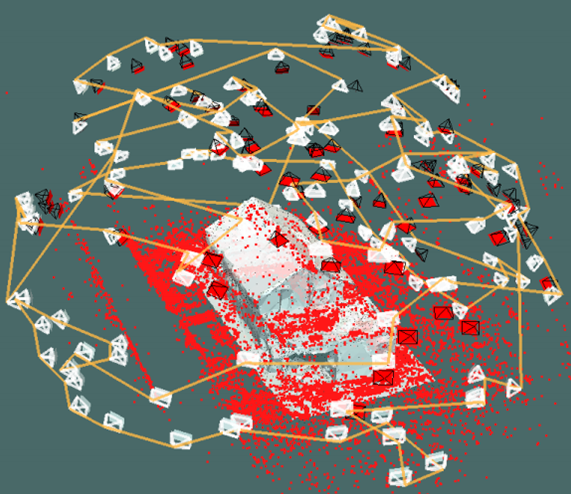
\includegraphics[width=\linewidth]{img/objectCoverFrom142.png}
  \caption{ Computed camera network pose estimation with the corresponding flight path (yellow) for an 3D object full coverage. This result is from Hoppe et al \cite{142*hoppe2012}.}\label{fig:ObjectCover142}
  \endminipage\hfill
\end{figure}

\begin{itemize}
\item Object coverage: \\
   %The definition of a coverage can be varied this is a good example. 
   In Hoppe et al \cite{142*hoppe2012}  a good coverage is defined by the ability to have full 3D reconstruction of an object (in their 3 dimension) with no occlusion. This definition of the coverage is exploits the prior knowledge of the object to cover. In this case the camera position will make a sphere around the object to cover as in the Figure \ref{fig:ObjectCover142}. 
   This definition of coverage is not the more helpful due to this restricted application, focused only on 3D reconstruction. This formulation and  consequently the solution proposed is not applicable for the area coverage.\\ 
   \item Path to cover: \\
   The coverage problem may be reduced as a series of paths commonly borrowed by the users (car, pedestrian, …). When the area to cover is a well-known place the path of the users can be deduced \cite{27*bodor2005} or if the area to cover is a road the trajectory of the driver is knew \cite{14*lu2011}.  In this condition, the aim is to cover the common path of the user as presented in  \cite{14*lu2011,27*bodor2005,30*bodor2005,81*nikolaidis2009}. The path coverage is interesting due to this numerous restriction on the area to cover. Thanks to the restriction the coverage may became easier. Otherwise the path coverage introduce an important element is the zone with has a priority. This restricted zone in the area have to be the only area taking in account or  at least  the area  cover in priority.\\
   \item Coverage priority: \\
   A natural way of defining the coverage in a context of insufficient number of cameras, is to define in priority some zone of interest to cover.
    In \cite{84*xu2011,165*jiang2010,171*horster2006}, their proposed to focus on priority on some predefined region, respectively called region of interest, curial sub-area (see Figure \ref{fig:MapRoI165}) and importance space weighting.  In the solutions proposed  by \cite{84*xu2011,165*jiang2010,171*horster2006}, the cameras poses are in priority affected to this specific and restricted region which has to effect too neglected the other part of the area. \\
Logically if the environment is described with some region of interest some neutral zone must exist. The neutral zones (or normal sub-areas) must be covered, but they are not the priority. Furthermore, some regions can be described as no interest regions. In \cite{165*jiang2010,171*horster2006}  for example, the obstacle are designed as non-interested region and also this region have as consequences to occlude the vision of the camera. The main interest of this design is to keep a maximum of the freedom in the cameras network positioning and see if the camera position can manage with the different local priority and constraints.\\
\item Inside or outside area:\\ 
Finally one of the simplest view of the coverage concern the outside and inside area coverage. The area to cover can be typically a room with walls. Each walls can be a considered as an obstacle and can occlude the camera field of view. In this case the main objective is to cover the surface in totality or at least maximize the coverage. This formulations is also workable for the vast outside area, but in addition it is necessary to take into account the size of the environment and the cameras limitation (as the depth of field), which can make the solution even longer and complex.
   
\end{itemize}
  


\begin{figure}[t!]
\center
\minipage{0.75\textwidth}
   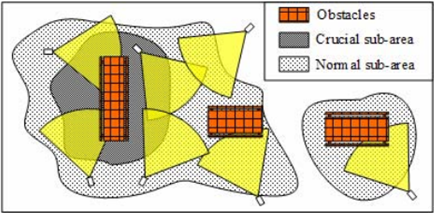
\includegraphics[width=\linewidth]{img/MapRoI165.png}
  \caption{ Map of an area to cover with crucial sub-area (region of interest) the normal sub-area  and obstacle. This map is an example of area coverage  introduce in  Jiang et al \cite{165*jiang2010}. }\label{fig:MapRoI165}
  \endminipage\hfill
\end{figure}

The common point in all this coverage definition is the importance to maximize it, despite the other objectives. In the examples presented the coverage was always the first and for some of them the only objective. Despite the interest for maximizing the coverage some other elements has to be taken in account to have a useful cameras position depending on the finality. The secondary objective can have a not negligible impact on the camera pose.  The secondary objectives are numerous and closely related than the finality. Among the secondary objective available with their numerous adapted version, some of the most interesting of them are presented :\\
\begin{itemize}
\item  The numbers of cameras: \\ In numerous situation, the secondary objective has to limit the number of cameras affected to the area as \cite{151*zhao2013,171*horster2006,22*zhao2008}. Limit the number of cameras is primordial to decrease the time computation for the final application and in some case the network traffic. Also reduce the number of cameras to cover the full area mean reduce the cost of the video surveillance installation as \cite{82*chrysostomou2012}. In the case  minimizing the number of camera is a secondary objective not directly in contradiction with the camera pose optimization for  best coverage. The two objectives can become complementary. At some point a too strong trade-off in favour of the minimizing the numbers of cameras may reduce the area cover by accepting some small area  non covered. The small area is know as black hole. Otherwise,  if the trade-off is in favour then the complete coverage of the area the risk is to have a too high number of cameras (with numerous overlap).\\

\item Object tracking: \\ The secondary objective can be after the area coverage, to detect and localize targets as for example in \cite{18*ding2012,12*soto2009,23*liu2009,39*wu2011,40*sohrabi2000,22*zhao2008}. In these cases, the secondary objective is to find cameras pose or dynamic adaptation of the pose for follow one or numerous targets. The dynamic adaptation is commonly adapted to the looking direction in order to track the target. The dynamic adaptation is applied on the network composed by PTZ cameras as in \cite{18*ding2012,38*liu2010,12*soto2009}.
Keeping a full area covered and at same time the when the secondary objective is to track efficiently one or more target, can become contradictory. The solution must be a trade-off, between the maximum coverage and the tracked track, as in \cite{18*ding2012} and \cite{38*liu2010}.
 In Liu et al \cite{38*liu2010} the tracking of a target in a wide area is decomposed in phases, detection and location phase. For the detection phase, the area coverage is important but not any more for the location phase. These phases, although distinct for one target can intervene at the same time if there is more than one target. Obviously when the secondary objective is to do tracking the cameras position will be less efficient to cover the area depending on the numbers of targets.  \\

\item  Luminosity and environmental setup:\\ Also  the  control of the image quality in terms of visibility can be an objective. Reddy et al \cite{33*reddy2012} are focussed  in a first time, on  the coverage of a complex area and in second time the targets localization. In order to manage what target must be followed the visibility is taking into consideration to avoid the too dark area, where the target is not enough visible at all. \\

\item  Energetic cost:
\\ To estimate the camera positioning another secondary element can be the energy cost in \cite{38*liu2010,42*bulusu2001}. Lui et al \cite{38*liu2010} is a good example, the first objective is to cover most of the area to be able to detect if a target is entered in the area to control. In a second time, the target is followed by  the smart and autonomous cameras of the network. The set of cameras were randomly dispersed in the area and the coverage of the area will be to select the cameras useful to detect the targets intrusion. The selection of the camera is managed between the maximum area coverage and the minimum cost consumption. In this case the consumption is reduced by reducing the number of smart camera turned in detection mode. In Lui et al \cite{38*liu2010} the smart cameras are considered has more or less greedy depending then mode activated (detection or tracking). Moreover the energy cost can be considered not only in term of number of cameras turn on, but also in term of distance between each cameras. Notably in the case of each camera position will be a waypoint for doing a path planning \cite{191*di2016,218*meiting2007}.  
\\
\item Multi coverage:\\ Among the numerous secondary objectives possible, the multi coverage is interesting (as for example in \cite{149*mavrinac2013,151*zhao2013,152*wang2009,174*zhang2016,175*medhi2013}). The multi coverage or also called $k$-coverage where $k$ represent the number of cameras useful to cover some region of the area. The multi coverage or $k$-coverage can be at some point confused with the region of interest and coverage priority (see more in detailed in section \ref{sec:zoneOfInterest}). Mostly due to their importance given at some restricted part of area. The difference between them is the impact of the multi coverage on the finale coverage. The multi coverage involved one or few specific zone of the area to be covered by a minimum of $k$ cameras at same time in order to be considered as cover. This secondary objective in the case of limit will generate a conflict between the full coverage of the area and the $k$-coverage requirement even more with a restricted number of cameras. 
\\ 
\item  Resolution:\\ The objective of resolution is to keep the quality of the image acceptable \cite{27*bodor2005,33*reddy2012,171*horster2006,152*wang2009,43*erdem2006}. Most of his article are used the distance along the optical axis as parameters in order to evaluate the resolution constraint. The lens, the sensor and the distance between the camera  and a target (or surface) is used to estimate the resolution. In many application is essayer to adapt the distance between the camera and the target or the zoom (when the lens is not a fix focal) then to modifies the other parameters as the sensor or the lens.\\
%The resolution is also model as the acceptable the depth of field.
  This secondary objective affect mostly the positioning system of a cameras set by comprising a zooming lens when the  number of cameras is fixed. Consequently, if the resolution constraint is not selected, the risk is to have all the cameras at the maximum zoom out (or place the camera highest) due to the optimization , in order to cover the wider region as possible. When the constraint of resolution is added a trade-off must be done between the zoom out (or the camera distance to the target) for maximizing the coverage, and the zoom in to reduce the area cover for a better resolution. The trade-off is particularly relevant when the number of cameras is slightly more important then the optimal need.
   In \cite{33*reddy2012} the resolution is assimilated to be part of the image quality. In order to keep enough quality on the followed target, the distance of the target is used to keep an acceptable resolution. The problem has been designed by using a Gaussian function in order to define the proper distance between the cameras and the target to keep an acceptable resolution for the application. \\
Also the depth of view has the same consequence on the camera positioning. Due to the focus point and the aperture of the camera (associate to the resolution), an object to close or to far became blurred. An ideal distance between the target and the camera is defined with some boundary as in \cite{193*fu2014}. % (find ref 193)

\end{itemize}

The secondary objectives are numerous and varied, where just few of them has been introduced (the more common and interesting). Among it, some of them are closely related and can be interconnected. The secondary objectives can be associate as in \cite{33*reddy2012} for example where the coverage target, luminosity, the resolution, and obstacle constraint are associate to find the best cameras position with maximize the coverage of the area and the  tracking target with good visibility condition. \\
The real interesting element about the secondary objectives is the impact in the cameras positioning for the global coverage of the area. Consequently the finality and the problem formulation will have a considerable impact of the obtained solution. Obviously the secondary objective have to be chosen carefully and there are related then the finality. To have an efficient cameras positioning system has to trade-off between the different objective and their importance have to be done in order to know what is the priority. In this case, the problem became a multi objective problems. 
The secondary objective can be considered as a constraint with can restrict the main objective which is the coverage of an area.


\section{Art gallery problem} \label{sec:AGP}
%Once the objectives defined the next step, is to know how to represent the problems. To do that manly 2 different class  of problems have to be studied. The first is from the geometrical problem called  the Art galery problms.

%The previous section was focus on the objectives definition as well as the finality around the sensors and cameras position

%Until now the problem was presented in term of objectives and constraint in order to be used in a concrete situation.

The Art Gallery Problem (AGP) is a theoretical and historical problem closely related than the camera positioning. The AGP is commonly cited  in the literature as a source of the problem and also used in the AGP paradigm is used to formulate the problem of camera positioning (as example \citep{44*chvatal1975,53*packer2008,149*mavrinac2013}). For these reasons the AGP as to be well understood before to go further.

%Until now the problem of coverage was studied to place cameras. The use of cameras (fix or mounted on mobile robot) are the limited field of view  and  depth field of the sensor. An interesting paradigm closely related is to use human guards  instead  of the set of cameras.  This paradigm is called the Art Gallery Problem (AGP). The AGP is an interesting  paradigm with propose some efficient solution. 

In the following section a definition of the AGP is given with a brief historic. Next to this introduction on AGP, some of the more interesting solution proposed are discussed before to see the limits of this paradigm.

%The problem of camera positioning is a tricky problem. The positioning of the set of cameras depend on many factor. To solve this problems is importatant to know more about the relat
% %finality of the camera networks and the formulation the camera pose will be affected.\\
%% Once the objectives defined ( see section \ref{sec:camerasPositioning}) the next step, is to know how to represent the problems. To do that manly 2 different paradigms have to be studied.
% The first is from the geometrical problem called the Art Gallery Problem (AGP) formulation is commonly and historically borrowed as is presents in the following section with a fast definition of the problems, the solution used and the limit of this paradigm.


	\subsection{Definition of the paradigm} \label{sec:AGPdef}
	The art gallery problem is a geometrical problem introduced by Victor Klee in 1973. The problem was to estimate the number and the position, of useful guard to cover an art gallery. 
The particularity of a art gallery is the complexity of the room shape, with many walls to dispose the painting. The shape complexity of the room make the estimation of guards number even more difficult.\\
In order to formulate properly the problem, the room is assimilated as a polygon $P$, composed by $n$ vertices ($v_1; v_2;…v_n$). The vertices are linked by $n$ edges ($v_1 v_2;…; v_{n-1} v_n$) to make the shape of the Polygon $P$ (or room).

A guard $x$ is inside the room $x \in P$. A guard $x$ can cover or see any point $y \in P$ if the segment $xy$ is not intersect by one of boundary ( a wall) of the polygon $P$, in order to have $ xy \subseteq P$.
The polygon $P$ is considered as fully cover when for any position of the point $y$ in the polygon at least one guard can see it .\\
A guard $x$ can have a $360^\circ$ field of view to cover all around him, with no depth of field limitation (except the wall obstacle). Clearly that mean the guard can see and monitor the entire length of the room one side to another side if no obstacle around to occlude. For example, if the shape of the room is a triangle, quadrilateral or another convex simple polygon, at any position taken by one guard, this guard can monitor all the area despite the size of the art gallery. 

When the polygon is more complex, it is necessary to estimate the minimum number $g$ of guards $x$ and the position of the guards $x$ in polygon $P$. 
 The set of minimum number of guards are listed in $X$. Where $X$ contain the useful $x$ to fully cover the polygons $P$, with $g$ the minimums number of guard in order to have a set of points $X=\{x_1…x_i…. x_g\}$. So that every point $y$ in $P$  are cover by at least on guard $x$ of the set of $X$. \\
The AGP in addition to estimating the numbers of guards also are interested on finding the optimal position of this restricted number of guards. 
This 2 questions can be solved at the same time by using one of the solutions proposed.


	\subsection{Solution }
	
	The advances on the AGP since this formulation in 1973 are numerous. The following paragraphs present the major advance on it.\\
	 The first and one of the more important is the proof given by Chvàtal in 1975 \cite{44*chvatal1975}.  The polygon must have to be covered by a minimum of guard, the proof of Chvàtal propose to link the minimum number of guards to the number of vertices $n$. 
A polygon composed by $n$ vertices need in the worst case a minimum number of guards equal at $n/3$. The Chvàtal proof is based on the triangulation of the polygon. The Triangulation is made based on the vertices of the polygon.\\
	 % For a polygon composed by $n$ vertices in the worst case the minimum guard necessary to cover it, is $X=n/3$.
	     The proof given by Chvàtal is also confirmed by the work of Fisk  few years later (1978). The work of Fisk is also based on triangulation and colouring node. It is probably the easiest to understand and also give a solution to estimate the pose of each guard. It is recommended to begin by the Fisk proof before the Chvàtal despite the chronology order as it is recommended in \cite{219*orourke1987}. The book of O'ROURKE et al \cite{219*orourke1987} is an early work about the AGP with the formulation, proofs and advancement of the field clearly explained. \\
Once the proof of the minimum number in the worst case founded the objective became to find an optimal guard position for all kind of polygon in reasonable time. \\
For that the work of Toussaint and Avis (in 1981) is the reference and propose a solution working in $O(n log n)$. This work has been follow and upgrade until the solution of Couto, Resend and Souza  2011 \cite{224*couto2011}. The solution  finally proposed work in $O(n^3)$ complexity in the worst case. 

%It is a short overview of the AGP solution but also the solution proposed are very specific to the AGP and cannot be re-use for problem little different.

	
	\subsection{Limit of AGP and camera coverage relation}

The AGP can be considered as a reduction of the problem of the best cameras pose estimation to maximize the coverage of a complex area. Based on the algorithm developed to solve the AGP and the strong relation between AGP and the cameras positioning for maximum coverage. It is logic to have some proposed algorithm which tries to extend the AGP to the  problem of camera positioning as example in \cite{221*fleishman2000,33*reddy2012,43*erdem2006}.

%The problem of positioning cameras for maximum coverage is quite close then the AGP. The AGP is a reduction of the camera positioning for a total coverage of a complex areas. The camera positioning is the logical continuation of AGP and once the AGP is solved , the problem can be extended as is for example show in \cite{221*fleishman2000,33*reddy2012,43*erdem2006}.

The algorithm developed for AGP cannot be applied directly on the problem of cameras positioning for maximum coverage. The main reasons are the cameras limitations as field of view and depth of field (see \cite{82*chrysostomou2012,170*yabuta2008}). The cameras limitation makes  unreadable the algorithm proposed to solve the AGP.
 Because the AGP considering the guard with no limitation for the depth of field and field of view. Due to these differences the geometric model of AGP may not be applicable for perspective camera.
Also another reason make the AGP solution not applicable for the camera positioning can be the diversity of cameras. In the same system the AGP may have many guard, they are all interchangeable because it has all the same ability (or skill) to monitor the area. In contrary it is possible to have for a cameras network different kind of cameras with different lens. 
Finally the  perfect assumption for the AGP formulation create important weakness when is time to replace the guards by cameras. These weakness make the algorithms form AGP not adapted in our problem, as is showed in \cite{81*nikolaidis2009,171*horster2006}.
%This weakness in the AGP formulation associate to the limited field of view  make the solution form AGP note adapted as  is showed in \cite{81*nikolaidis2009,171*horster2006}.\\Due to this limitation, the solution developed for AGP are not applicable. 

However, some part of the AGP formulation and especially some proof has their importance, as the proof of Chvàtal \cite{44*chvatal1975} or the NP-hard complexity proof. 
In fact the AGP is NP-hard problems \cite{219*orourke1987}. The NP-hard proof is available on the book of O’Rourke section 9.2 of the book \cite{219*orourke1987}. 
To proof the AGP is  NP-hard, the first part is to reduce the  problem to an other problem well known for this complexity. The relation is made by reducing the AGP with a polygon composed by  holes to another standard problem (in the demonstration the 3SAT is used to be exact). 
Once the AGP is reduced to 3SAT and because 3SAT is an NP-complete problem the AGP is  also considered as NP-complete or  NP-hard but only  when the room is composed with holes. Also another work of Lee and Lin 1986 proof the complexity of AGP without hole also by reducing the AGP ton an other well known problem (for more explication see the book of O’Rourke  section 9.3 \cite{219*orourke1987})).
Despite the limit of AGP, numerous article are based on the AGP to formulate the problem as in \cite{43*erdem2006,53*packer2008}. For example in \cite{43*erdem2006} a similar approaches then the AGP is used in order to estimate the occluded region. 
As we explained earlier the camera positioning can be reduced as an AGP \cite{53*packer2008} notably by removing most of the constraint due to the camera properties. 

In the literature numerous article use the AGP as reference to explain the complexity of the problem as for example \cite{26*moeini,44*chvatal1975,149*mavrinac2013,151*zhao2013}  assumed the problem is at least NP-complete or NP-hard. 
The complexity of the problem will have an impact on the solution used  to try to solve it and optimize it.\\
One other impact of AGP in the problem of camera positioning is the shape of the room. In \cite{170*yabuta2008,171*horster2006,33*reddy2012,43*erdem2006} the shape of the room to cover are close then the definition of an art gallery. The art gallery room is a complex polygon composed by many vertices which may occlude the view. This phenomena can be imputed to the link did between the number of vertices and the useful number of guards to cover it. 
In addition the occlusion formulation made for the AGP is commonly used.
The occlusion in AGP is defined  by  a segment $xy \not\subset P$   where $x \in P$ is the guard position $y \in P$ is a points in the room $P$. 
Moreover the use of a complex room inspired by AGP is therefore a good choice in order to verify the effectiveness of the algorithms developed for the camera positioning in a complex environment.
%The complexity of this problem is also an important factor which makes the relation of camera positioning and AGP. \\


The AGP can be at same time for part, the  historical source of the cameras positioning and give some beginning of answer about the problem, this formulation and this complexity. Despite that, the AGP is not the only source to refer about the cameras positioning for maximize the coverage. Some clue and algorithm can be found in other related field. 


\section{Wireless sensor network }

The Wireless Sensor Network (WSN) can be as AGP considered as inspiration for the  of cameras positioning for maximize the coverage. The WSN is an active field of research and in many aspects related to the cameras positioning. This parties is focused on the WSN and this relation with the camera positioning.  To begin:

\textbf{ What is the Wireless Sensor Network (WSN)? }

 The WSN is a distributed network of sensors or in some case actuator, in this case is also called WSAN. Each sensor of the network is a relay for the information and commend, to the rest of the network.  
The sensor are at same time the node and the relay for the network. The node has to objective to transmit by relaying the information to the other node. 
The information can be centralized or not :
\begin{itemize}
\item When the system is centralized the information has to be transmit node by node until the centralized agent.
\item Otherwise the node have to be the sensor for collect information and decided to communique with the other node depending then the situation. 

\end{itemize}
 
The information collected by the sensor are vast depending on the final application and the capacities of the sensors ability. 
The WSN is used in different field for various application as for Telecom with antenna positioning \cite{59*wang2008}, military surveillance field \cite{38*liu2010,101*topcuoglu2009}, airport surveillance \cite{37*ma2012}, video surveillance and tracking \cite{38*liu2010}, environmental monitoring \cite{42*bulusu2001}... 
Logically numerous sensor and information can be collected depending then the need as temperature, movements, images, song and also some  actuator can be used as radio frequency for example.\\
 The application of WSN are wide, especially since the WSN has more than one discipline. The WSN try to optimize a network of sensor in different aspect as for example \cite{39*wu2011} focus on an architecture adapted and efficient enough for data transfer (here the data are images) or like in \cite{40*sohrabi2000} the WSN are dedicate to adapt the network around static node and energetic resources in order to keep the network connected.  \\
For our case the aspect the more interesting of the WSN, is the coverage of an area with his specific constraint and secondary objectives.
 The other discipline of the WSN as the network optimisation will not be addressed in the following document. Only the problem of coverage is studied the other discipline are not considered as the first or main objective but can be some secondary objectives after the problem of coverage which has to be taking in account for the optimization. 

\subsection{Sensor at 360}
%
	\begin{figure}[t!]
	\center
\minipage{0.55\textwidth}
   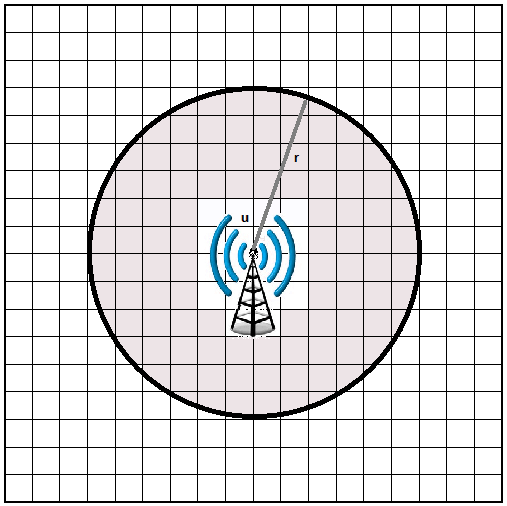
\includegraphics[width=\linewidth]{img/WsnSensor1.png}
  \caption{ One omnidirectional sensor centred on $u$, with a radius $r$ for the range.}\label{fig:WsnSensor1}
  \endminipage\hfill
\end{figure}

The WSN refer commonly to sensors or actuators  with no restriction in the view angle, it is considering to have a $360^\circ$ field of view. The sensor Field of view can be represented in a 2D plan  as in \cite{200*kulkarni2011, 174*zhang2016,150*chakrabarty2002} (as illustrate in the Figure \ref{fig:WsnSensor1}) and in some case a spherical for the 3D environment example in \cite{175*medhi2013,59*wang2008}.  

Each sensors have a position $x$ in the area and a power range. From the sensor power  the radius $r$ of the circle is deduced from $x$ as center (show \ref{fig:WsnSensor1}). This circle give the area cover by a sensor in the simplest case. 
The simplest case correspond to a flat area without any obstacle, or it is negligible with do not impact the covered area as in \cite{200*kulkarni2011,174*zhang2016}.  
Others more complex solutions can be used. Its are more complex but also more realistic as in Wang et al \cite{59*wang2008}. Where are taking in account the relief and obstacle. 
In Zhang et al \cite{174*zhang2016} more complex model have been developed, where despite of a flat ground without obstacle each sensor is composed by a perception radius and a communication. The communication radius a bit bigger then the perception radius. This 2 radius correspond to area covered for one antenna (sensor) and the distance of emission/reception of the data.  In order to have an efficient coverage of the area, the antenna must be place in order to have connection with other antenna but without too much overlap of the perception sensor.\\

The solution proposed in order to optimize the positioning of the WSN for a circular sensor can be varied. Mostly 2 different ways are applied for the sensor with have circular angle of view or spherical.\\

\begin{itemize}


\item	The first solution use an heuristic based on geometry construction as in  Medhi et al \cite{175*medhi2013}. This approaches give a good coverage solution but is usually greedy and can be quickly limited in term of number of sensors. Moreover if some external constraint are added.  For example in zhang et al \cite{174*zhang2016} the greedy solution was tested and optimized by using a "partition and shifting" strategy in order to upgrade the result.
The limit of this solution despite the greedy consumption resources is also not applicable to the problem of camera positioning due to the reduced field of views of a cameras.  \\
\item	The second solution, try to find an efficient and quick solution to optimize  random position for each sensor of the network.  
This solution include many different family of algorithms focused on optimization.
Among the family of algorithms, the evolutionary algorithms (disused in detailed in section \ref{chap:EA}) is commonly used as in \cite{200*kulkarni2011,59*wang2008}, and \cite{150*chakrabarty2002}. \\
These solutions propose to optimize the position in order to maximize the coverage depending on constraints and the secondary objectives. The method of optimization have to be adapted to the problem. 
In Chakrabarty et al \cite{150*chakrabarty2002} the integer linear programming with an "LPsovlver" are chosen in order to maximize the coverage with 2 type of sensors. One standard with a smaller area coverage but with a smaller cost (can have a $100m$ radius for 150\$) and the other sensor can cover a wider region (can have a $200m$  radius for 200\$) and the objective is to cover the region with a second objective is to reduce the cost. The solution proposed is to use the integer linear programming adapted to the problem of coverage optimization with the economic cost as constraint. \\
In \cite{59*wang2008} and \cite{200*kulkarni2011} the solution proposed is based on 2 different evolutionary algorithms in order to optimize the sensors positioning. 
In kulkarni et al \cite{200*kulkarni2011} the camera positing with a multi coverage is solved with using an evolutionary algorithm called Particles Swarm Optimization (PSO). The objective is to optimize the position of the sensor in order to have an efficient coverage of the area and also enough redundancy to keep the network workable if one or few sensor fail. In Wang et al \cite{59*wang2008} one evolutionary algorithms is also used to optimize the position of antennas. The objectives in this paper is to give the best coverage of an area with taking in count the relief of the area. The relief make the coverage estimation of each sensor even more complex and costly in terms of time computation. The Genetic algorithm are used in order to find quickly a position for each antenna of the network. 
\end{itemize}

Among the solution proposed, the second, based on optimize a set of sensors position  depending then  the constraints, is the more interesting and the more flexible to the add of new constraints (and secondary objectives). 
Now the following section  is dedicated to see if this solution is applicable to the problem of positioning a set of cameras. Despite the camera constraints.
%The aim is to see up to what point and if it is applicable to the problem of cameras network positioning.  

	\subsection{Visual sensors}
	
Logically, the result obtained with the Omni-directional sensors are interesting and must be applied to the problem with even more constraints and objectives as can be the positioning of visual sensor network (VSN). The term of  visual sensor contains several types of cameras with several constraints and properties. Despite these several type of cameras, the more commonly used and studied is the perspective camera (as in \citep{149*mavrinac2013,174*zhang2016,193*fu2014,42*bulusu2001}). 
  In fact the visual sensor or camera have a limited depth of field but also a limited field of view. This new constraint makes the cameras positioning more complex, as that was for AGP (see section \ref{sec:AGP}) to passes from guard to camera.
 The advantage in these cases, are first the sensor has been designed with a limited depth of field (the sensor has a limited power range). 
 Moreover the solution applied previously for circular sensor was not only geometric or based on heuristic algorithms. The problem has also been formalized as an optimization problem. These problem formulations allow to use optimization algorithms and meta-heuristics. In addition, these problems formulations appear as the more suitable to add constraint and secondary objectives. Thanks to that, the solution  developed for the WSN can mostly be adapted to the problem of camera positioning. 
 The following sections as to aims to disuse about the algorithms applied until now to the problem of camera positioning.
 %but also the problem is formalized as optimization problems with some solutions based on optimization and meta-heuristic. This way to present the problem is appear as the more suitable to add constraint and secondary objectives. Also the solution and the formulation for the problem of VSN are mostly the same then the problems of cameras positioning and is discussed in the following parts  \\
  

	\section{Solution not based on evolutionary method}\label{sec:NonEAmethod}
	
The algorithm used to pose a set of cameras in order to maximize the coverage are various.  Among the possible algorithms manly two families can be describe. The algorithms proposed they come from numerous sources and paradigm  which AGP and WSN.\\
 The first family is to construct a solution using an heuristic to have an appropriated cameras position. The second way is to formalize the problem as optimization problem and applied meta-heuristic. 

\subsection{The constructive solution}

The cameras pose can be done by construction. By construction that mean a deterministic method is applied to pose iteratively one camera after the other  or to adjust their positions based an initial set-up.\\
In Liu et al \cite{38*liu2010} a constructive solution is applied in order to select the smart cameras of the network. Each smart camera are a node of the network and transmit informations, images. The smart cameras are fully autonomous in term of energies and decision making ability (no central master). 
They work in 3 different modes:
\begin{itemize}
\item[-] The first is the sleepy mode. The sleepy mode is used in order to economize a maximum of the energy. To do that the camera is turn off. That mean no computation and just the network is listen at regular intervals to wait the wakeup call.   \\

\item[-] The Second is the detection mode the camera is turn on, but with a low frame rate. Just a few computation is done to detect if a target is enter in the field of views. Some information may be transmit by network. This mode consume more energy of the previews but the smart cameras can stay in this mode during a long time.\\

\item[-] The last mode is a tracking mode. This mode is the more energy consumer. The camera is turn on, with a high frame rate and numerous computation are done to track and localize the target. Also more information have to be transmit by the network. The information are useful to localize the target by communicate with the potential other smart cameras with have a view on the target. 
\end{itemize}

The objective in \cite{38*liu2010} are multiples, depending on the state of the cameras. The one the more interesting for us is to keep under control the longest time as possible the area for target detection. Numerous smart camera are randomly dispersed in the area (as an air-drop in a battlefield) and the aim is to select the cameras in order to maximize the coverage of the cameras turn on detection mode. The solution proposed by Liu et al in \cite{38*liu2010} is to use a constructive algorithms. The network of camera self-recognized  by a talk between each smart cameras. Also each smart cameras is able to estimate precisely this localization, it is an important assumption to select the cameras. The solution proposed is directly inspired by the distributed network talk. \\
To begin all sensor are in sleepy mode. The camera wake up regularly and send a call at the neighbour, if they receive no answer that mean no other camera is awake around and the camera stay in detection mode. If no enough answer have been received, that mean the required density of the camera around are not enough the camera stay turn on detection mode. Otherwise the camera return on sleepy mode until another wake-up later. This procedure is applied in each smart camera with all have their own pace. After a certain time the network is well organize to cover the area in detection mode. The area is considered covered when the density of camera is good enough. \\
 The method introduce by Liu et al in \cite{38*liu2010} is efficient enough. The solution proposed have the advantage to can work in wide area and to be dynamic as example if a camera do not have any more power the network will self-recognize.  
This algorithms is efficient with a high density of sensor to have a relatively low coverage (just enough to detect target in the sparse sensor placement). Also the method presented is really dependent then the network communication and the capability to localize precisely each sensor. Finally the solution proposed to select a set of sensor among a randomly posed sensor is not enough optimized and precise.

Another cameras pose estimation by construction is proposed by Höster et al \cite{171*horster2006}.
The solutions proposed is based on a greedy search heuristic. The objective is to find a position and orientation of a set of cameras with a fixe pan, in the environment inspired by the AGP. \\
In \cite{171*horster2006} a first greedy search solution has been presented before an other algorithms with extend the greedy solution. The algorithms developed in \cite{171*horster2006} is called Dual Sampling.\\
The dual sampling is an incremental method. 
First step, is to initialize the position of all the cameras. A random initialization for the position and the orientation must be appropriate.  \\
Second step, is to select one point of the area non covered yet. The area is discretized by several points, with each point must be covered by at least one camera. Around the selected point several position and orientation are tested for the cameras at proximity. The possible position are obtained by sampling the area around the point to cover. Finally the best cameras position and orientation is kept. The best camera position and orientation depend then the number of other points globally covered in the area. 
The second step is repeated and the set of uncovered control point is reduced at each iteration. This procedure is applied until the stop criterion is reach that mean enough points of the area are covered. \\
This constructive solution have some inconvenient notably in terms of efficiency. Indeed this solution is limited by the number of camera and size of the area due to the exponential complexity. %In fact, bigger area mean more point and more camera mean more position and orientation to test at each iteration.

In Nikolaidis et al \cite{81*nikolaidis2009} the cameras placement is studied for cover a basic mobile robot trajectory.
The trajectory of the mobile robot is modelled as the region of interest, with a gradually decreasing interested from the trajectory center.\\
  The solution applied in \cite{81*nikolaidis2009} is to do a local optimization one camera after the other with the “steepest decent method (decent de gradient)”. If this local optimization give a better solution the network of camera is modified otherwise the camera stay at the same place. This operation is repeated until the convergent arrangement is obtained or no more upgrade can be found. The result presented in the experiment done by Nikolaidis in  \cite{81*nikolaidis2009} are interesting despite the simplicity of the area and the very small amount of camera used (no more then four). The principal limitation is due to the number of steps required for optimize independently each camera of the network. Also a multitude of local optimisation is not obviously the same or better then the global optimization.

Ma et al \cite{37*ma2012} propose a solution for the problem of finding the minimum cameras barrier coverage. The objective is to cover only the boundary of an area, to be able to detect target intrusion in the perimeters. The perimeter is relatively wide and can be considering at some point as an area to cover composed by big hole in this center.\\
 The region to cover is cut in numerous sub-region. The region are inter connected, each sub-region have to be “full-view covered”. The full-view covered is defined ; if for any target direction there always exist a sensor cover to the face of it.\\
The solution purposed is based on constructive solution with adapted heuristic. The heuristic used is presented in detail in \cite{37*ma2012}. The global idea is to cut the perimeter in different sub-region and applies the method proposed to have a full-view coverage at each sub region. 
The cutting on sub-region offer at the heuristic to work in reasonable time due to this restricted area.\\
The solution proposed though this efficiency in the case of barrier coverage is not rely appropriate to vast coverage area. The first limitation is the number of cameras use to fully cover the area. The important number of cameras is mainly due to this definition of “full view covered”. That definition imply many overlap to have the multi direction coverage.\\

The previous solutions and algorithms presented in \cite{38*liu2010 37*ma2012,81*nikolaidis2009,171*horster2006} are based on constructive method for the cameras placement and their local optimization. Each camera is individual placed dependently then the network with an iterative process. The iterative process has to chose the best position for each camera of the set. This methods has some consequence, nobly the fast increasing number of iteration required to have a solution good enough for each camera. The time complexity is event more problematic with increasing the size of the area and even more with the number of cameras. Also these solution are extremely dependent then the formulation and the constraints and cannot be easily adapted to other problems or external constraint. The rigidity of adaptation is mostly due to the  use of heuristic  design for  very specific problems. 

\subsection{  Linear programming optimisation and limits}
	Different method of linear optimization was applied and test. In some case, due to a well-adapted formulation; a specific shape of the area or cameras number the linear optimisation is efficient. 
	The linear optimisation has been tested to have initial result in order to have a reference point before to develop other solution more appropriate(as example \cite{,151*zhao2013,82*chrysostomou2012}…).  
%	The reason ofIn some other case the method was studied but finally rejected du to this fast limitation 
	 The linear optimisation  is finally rejected due to this fast limitation.  Indeed the linear optimization can be quickly in difficulty due to the fast increasing complexity of the problem and in many case be locked in local minima. as presented in the flowing example.\\

%%\textbf{!!!!!! partie manguante sur l'utilation des methode linear  !!!!!(voir path planning)}
% non linear	 141*akbarzadeh2013,33*reddy2012 
	 \subsubsection{Linear programming}
In Erdem et al \cite{43*erdem2006} is based on AGP and the WSN and propose a fusion off their 2 paradigms in order to use there assumptions. Some modification have been done as example to take in account the field of view limitation. The interesting aspect is how some camera properties have been modelled to fit to the problem of AGP.  \\
The solution proposed being workable with using an omnidirectional or considering a PTZ as omnidirectional cameras by using an efficient angular sweep. The simile omnidirectional cameras are simulated by PTZ camera with a non-continue zoom or fix focal length as in the  experimentation proposed in \cite{43*erdem2006}.  Where the PTZ can have a focal two focal lengths at 50mm and  35mm. 
Finally the solution proposed is to discretize the area to cover and also the different possible parameter for the camera (as: localization, orientation, focal...) in order to have a combinatorial formulation of the problem. Thanks to this formulation close than the Binary Integer Programming (BIP) and apply a well-known method “Branch and Bound” in order to optimize the camera placement.  \\
This solution  proposes a  good  coverage with the minimum of cameras in a reasonable time. The limit of the solution is due to  the  use of omnidirectional or  simile omnidirectional cameras.% until, the  number of location sample, the numbers of cameras, and the number of parameters possible for the camera stay relatively  reduced.  \\
 
Zhao  et al \cite{22*zhao2008} are trying to find the optimal position for a set of cameras in order to maximize an indoor area coverage (similar than an AGP room). The coverage of an indoor area is not the only objective, but the requirement to can  do an efficient tag detection.
The solution proposed for the coverage is to adapt the number of points of interest which must be covered by the camera depending than the coverage rate. \\
The area is discretized with a grid.  The grid is composed by point selected smartly. Each point of the grid simulate a potential location of the target.
The camera position is limited at few position fixed on the room boundary.
% number of possible position for the camera (the boundary of the room) are defined.
The adapted grid and the limited cameras positioning are used to limit the size of the search space (as number of possible solution). Thanks to this limited search space a linear optimization with the Binary Integer Programming (BIP) can be used. \\
Use a BIP is popular and others use it as in \cite{22*zhao2008,43*erdem2006}. In \cite{22*zhao2008} the solution proposed is to use BIP formulation the grid smart sampling and branch and bound form LP\_solve libraries to optimize the camera position and orientation.\\

% A Similar method is used in \cite{27*bodor2005} to find the position and orientation of a set of cameras. The goal of this paper is to find the appropriate position with maximize the resolution for a set of cameras dedicate to do tracking. The position is determined depending on a set of standard pedestrian trajectories. The camera pose try to maximize the given trajectory to have the best resolution and the entire coverage. \\
%The problem is also formulate in order to apply a linear well-known algorithm. In this case the branch and bound is applied.  

\subsubsection{Limitation of linear method}
The methods of linear optimization were applied and tested to answer the problem of camera position for maximum coverage. In some case, due to a well-adapted formulation or a restricted area and cameras number, this solution is efficient enough. In some other case the method was studied, but finally rejected due to this fast limitation (as example \cite{141*akbarzadeh2013,151*zhao2013,82*chrysostomou2012}). Indeed the linear optimization can be quickly in difficulty due to the fast increasing complexity of the problem and in many case be lock in local minima.

In Wang et al \cite{181*wang2017} propose a solution with an atypical problem formulation. The solution proposed in \cite{181*wang2017} is mainly based on the method of discretize the area. The idea is to have an area discretized with precision with use the minimum of point. To do that the solution proposed is to decompose the area in order to give more point in the grid was the shape of the room need it to be correctly described. \\
The principal advantage of this solution is to propose an area representation with enough precision and a minimum of point to describe it. Less point to describe the area to cover mean also a winning time efficiency in computation during the camera pose estimation (cost function is faster).
Despite this interesting solution the result presented in the experiment does not appear to be conclusive.  

The principal problem of the linear optimisation appears when the problem became complex. The complexity can come form the  problem formulation and some extra constraint. But most of the time the increased complexity is coming from the increased size of the search space. Concretely when the goal is to place a more important number of cameras or when the number of positions and orientation are too important. 
	
\subsection{Game theory} 
	 
Among possible solution an atypical method is to use the game theory \cite{19*li2013}. The game theory is use to optimize the looking direction of the cameras as in \cite{12*soto2009,18*ding2012,19*li2013,25*song2008}. These articles are based on game theory to find an equilibrium (also named Nash equilibrium) between two contradictory objectives. The objectives are in one side toe maximize the resolution and  in the other side the multi target tracking.\\

Soto et al \cite{12*soto2009} propose a network of a dozen of PTZ cameras. The PTZ is for pan, tilt, zoom, that mean the position of the cameras are fix and the solution proposed is to find the best orientation with the appropriate focal lens to track most of the targets.  \\
 To do that the camera are smart enough to communicate with the close neighbours and adapt the pan, tilt, zoom depending on the needs.\\
The need has been defined by an utility function (or local cost function). The goal is to track most of the target as possible with the better resolution. The cameras scores when it obtained a desired resolution image for all the targets visible by the networks.\\
The trade-off proposed is between the multi tracking and the best coverage resolution for each target. The multi-target problematic can appear far from maximization of the coverage. But the number of targets which may be higher than the number of cameras, push the camera tracking to be an interesting solution to maximize the coverage of an area. In this case, the quality of the coverage will also dependent then the number of targets and the importance of the resolution constraint.  \\
	 In \cite{18*ding2012} and \cite{25*song2008} different experiments have been proposed with a number of targets  lightly increased. In this articles the game theory is applied to trade-off between the tracking and the resolutions. The proposed experiment is based on the decentralized method. It is justified by the complexity to dynamically adapt all the camera of the network at same time depending on each targets trajectories.\\
	  Furthermore, the decentralized solution is more adapted for the security of the transmission and the risk of interception by a hostile opponent. The security may be an important factor in some applications. \\
To have the decentralized system the cameras must have some autonomy. \\
In the experiment proposed in \cite{12*soto2009} and \cite{18*ding2012,25*song2008} each camera are smart enough to have their own tracking and control module. Also the camera are able to communicate with each other to reach until a consensus. The consensus is when a Nash equilibrium is found between the 2 contradictory objectives. In this case it is a win win situation for both objectives.\\
So the objectives are not independently optimize, moreover the solution proposed is to optimize its  simultaneously in order to have a consensus. The consensus is reach when it became impossible to upgrade one of them without downgrade the other one.\\
  In the experiment of \cite{18*ding2012,25*song2008} the consensus is found by the cameras communication. The cameras communication have to maximize numbers of  target covered with the higher resolution.
 The experiment is based on numerous targets moving freely in the area. Also in \cite{18*ding2012} one of the target must be cover in priority with a high resolution. That have an impact on the other camera position.
 The result of the experiment as in figure \ref{fig:CoverageFrom18} form \cite{18*ding2012} show a really efficient global coverage with almost all the target cover at every time despite the movements of the targets. \\
 The advantage of these solutions is the acceptable result and dynamic reconfiguration of the system for the reasonable size of the area and the decentralized computation.
 
Otherwise this method have some limit, as show in the experiment the area is relatively restricted and numerous cameras with a fixed position are useful. The consequences is the quantity of overlap relatively important. In this case the number of sensor is not well optimize to cover the area. Also to use properly this method for maximum coverage it requires a large number of simulated target in the region to observe.  Finally this solution is more adapted for a self-reorganization of the a set of PTZ cameras.

\begin{figure}[t!]
\center
\minipage{0.55\textwidth}
   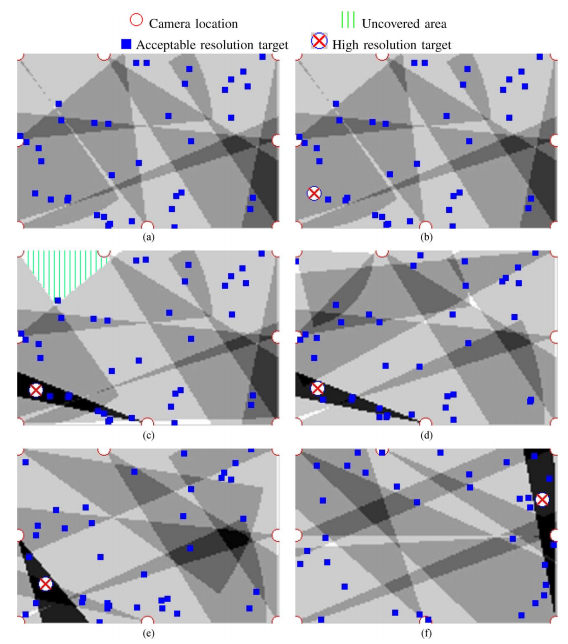
\includegraphics[width=\linewidth]{img/CoverageFrom18.png}
  \caption{ Result of coverage after have used the game theory with objective to maximize the tracking and the resolution. Result obtained in the experiment presented in \cite{18*ding2012}.}\label{fig:CoverageFrom18}\endminipage\hfill
\end{figure}
	
	%%%%%%%%%%%table sum up%%%%%%%%%%%%%%%%%%%%%%%%%%
	% Please add the following required packages to your document preamble:
% \usepackage{booktabs}
% \usepackage[table,xcdraw]{xcolor}
% If you use beamer only pass "xcolor=table" option, i.e. \documentclass[xcolor=table]{beamer}
%\begin{landscape}
%
%	\begin{table}[]
%\centering
%\caption{Sum up articles.}
%\label{my-label}
%\begin{tabular}{@{}lp{2.6cm}lllp{1.6cm}p{1.6cm}llp{1.3cm}p{1.3cm}p{1.65cm}p{1.6cm}p{1.3cm}p{1.3cm}p{1.4cm}@{}}
%\toprule
%\multicolumn{1}{|l|}{\textbf{ref}}               & \multicolumn{1}{l|}{\textbf{\begin{tabular}[c]{@{}l@{}}Best \\ solution\end{tabular}}} & \multicolumn{1}{l|}{X} & \multicolumn{1}{l|}{Y} & \multicolumn{1}{l|}{Z} & \multicolumn{1}{l|}{\begin{tabular}[c]{@{}l@{}}Point\\  selection\end{tabular}} & \multicolumn{1}{l|}{Pan} & \multicolumn{1}{l|}{Tilt} & \multicolumn{1}{l|}{Roll} & \multicolumn{1}{l|}{focal lenght} & \multicolumn{1}{l|}{\begin{tabular}[c]{@{}l@{}}Coverage\\  representation\end{tabular}} & \multicolumn{1}{l|}{\begin{tabular}[c]{@{}l@{}}number of \\ cameras\end{tabular}} & \multicolumn{1}{l|}{\begin{tabular}[c]{@{}p{1.65cm}@{}}Secondary objectives \\ and contraints\end{tabular}} & \multicolumn{1}{l|}{} & \multicolumn{1}{l|}{} & \multicolumn{1}{l|}{} \\ \midrule
%\rowcolor[HTML]{FFFFFF} 
%\multicolumn{1}{l|}{\cellcolor[HTML]{FFFFFF}37*} & heurisitic                                                                             & x                      & x                      & 0                      & 0                                                                               & x                        & 0                         & 0                         & fix                               & 2D                                                                                      & around 10 (per section)                                                           & barrier coverage                                                                                    & conection dependance  &                       &                       \\
%\multicolumn{1}{l|}{\cellcolor[HTML]{F2F2F2}38*} & \cellcolor[HTML]{F2F2F2}heuristic                                                      & \cellcolor[HTML]{F2F2F2}0                      &\cellcolor[HTML]{F2F2F2} 0                      &\cellcolor[HTML]{F2F2F2} 0                      & \cellcolor[HTML]{F2F2F2}\begin{tabular}[c]{@{}l@{}}random \\ dispersion (x;y)\end{tabular}              &\cellcolor[HTML]{F2F2F2} 0                        &\cellcolor[HTML]{F2F2F2} 0                         &\cellcolor[HTML]{F2F2F2} 0                         &\cellcolor[HTML]{F2F2F2} fix                               &\cellcolor[HTML]{F2F2F2} 2D                                                                                      &\cellcolor[HTML]{F2F2F2} around 600                                                                        & \cellcolor[HTML]{F2F2F2}resolution                                                                                          & \cellcolor[HTML]{F2F2F2}tracking              &  \cellcolor[HTML]{F2F2F2}                     &                      \cellcolor[HTML]{F2F2F2} \\
%\rowcolor[HTML]{FFFFFF} 
%\multicolumn{1}{l|}{\cellcolor[HTML]{FFFFFF}27*} & non-linear                                                                             & x                      & x                      & 0                      & 0                                                                               & x                        & 0                         & 0                         & fix                               & 2D                                                                                      &                                                                                   & tracking                                                                                            & resolution            &                       &                       \\ \rowcolor[HTML]{F2F2F2}
%\multicolumn{1}{l|}{ \cellcolor[HTML]{F2F2F2}43*} & \cellcolor[HTML]{F2F2F2}game                                                           & x                      & x                      & 0                      & 0                                                                               & x                        & 0                         & 0                         & x (discret)                       & omni directional (mobil pan)                                                             & around 10                                                                         & cost reduction                                                                                      & resolution            & DoF                   &                       \\
%12*                                              & game theori                                                                            & 0                      & 0                      & 0                      & 0                                                                               & x                        & x                         & 0                         & x                                 & 2D                                                                                      & around 10                                                                         & resolution                                                                                          & tracking              & multi target          &                       \\
%\rowcolor[HTML]{F2F2F2} 
% 18*                                              & game theori                                                                            & 0                      & 0                      & 0                      & 0                                                                               & x                        & x                         & 0                         & x                                 & 2D                                                                                      & around 10                                                                         & resolution                                                                                          & tracking              & multi target          &                       \\
%25*                                              & game theori                                                                            & 0                      & 0                      & 0                      & 0                                                                               & x                        & 0                         & 0                         & x                                 & 2D                                                                                      & around 14                                                                         & resolution                                                                                          & tracking              & multi target          &                       \\
%\rowcolor[HTML]{F2F2F2} 
%81*                                              & heurisitic                                                                             & x                      & x                      & 0                      & 0                                                                               & x                        & 0                         & 0                         & fix                               & 2D                                                                                      & 2 to 4                                                                            & Region of interst                                                                                   & trajectory coverage   &                       &                       \\
%22*                                              & LP-solve                                                                               & x                      & x                      & 0                      & 0                                                                               & x (16 orientation)       & 0                         & 0                         & fix                               & 2D                                                                                      & around 10 (8-11)                                                                  & tag detection                                                                                       & tag visbility         &                       &                       \\
%\rowcolor[HTML]{F2F2F2} 
%170*                                             & linear programming relaxation                                                          & x                      & x                      & 0                      & 0                                                                               & x                        & 0                         & 0                         & fix                               & 2D discret square                                                                       & around 20                                                                         & Region of interst                                                                                   &                       &                       &                       \\
%171*                                             & LP-solve                                                                               & x                      & x                      & 0                      & 0                                                                               & x                        & 0                         & 0                         & x (discret 3)                     & 2D                                                                                      & around 10                                                                         & cost reduction                                                                                      &                       &                       &                       \\
%\rowcolor[HTML]{F2F2F2} 
%181*                                             & Multistage Grid Subdivision                                                            & x                      & x                      & 0                      & 0                                                                               & x                        & x                         & 0                         & x                                 & 2D                                                                                      & 9 to 15                                                                           & Region of interst                                                                                   & big area              &                       &                       \\ \cmidrule(r){1-13} \cmidrule(l){16-16} 
%\end{tabular}
%\end{table}
%	
%\end{landscape}	
	
	
	%%%%%%%%%tab v2 %%%%%%%%%%%%%%%%%%%%%%%%%%%%%%
\begin{landscape}	
	\begin{table}[]
\centering
\caption{Sum-up ref}
\label{tab:sum-up1}
 %              ref           |x|y |z| pan|      tilt| |focal  coverage     nmb   
\begin{tabular}{@{}l|p{2.4cm}  l  l l p{0.659cm}p{0.62cm}lp{1.3cm}p{1.57cm}p{1.5cm}p{1.6cm}p{1.3cm}p{1.2cm}@{}}
\toprule
\multicolumn{1}{|l|}{\textbf{ref}} & \multicolumn{1}{l|}{\textbf{\begin{tabular}[c]{@{}l@{}}Best \\ solution\end{tabular}}} & \multicolumn{1}{l|}{X}              & \multicolumn{1}{l|}{Y}              & \multicolumn{1}{l|}{Z}             & \multicolumn{1}{l|}{Pan} & \multicolumn{1}{l|}{Tilt} & \multicolumn{1}{l|}{Roll} & \multicolumn{1}{p{1.29cm}|}{focal lenght} & \multicolumn{1}{l|}{\begin{tabular}[c]{@{}p{1.55cm}@{}}Coverage\\  room\end{tabular}} & \multicolumn{1}{l|}{\begin{tabular}[c]{@{}l@{}}number\\ of \\ cameras\end{tabular}} & \begin{tabular}[c]{@{}l@{}}Secondary objectives \\ and constraints\end{tabular} &                      &               \multicolumn{1}{l|}{} \\ \midrule
\rowcolor[HTML]{FFFFFF} 
\cite{37*ma2012}   Ma 2012                     & heuristic                                                                             &  \ding{52}                                   & \ding{52}                                   & 0                                  &  \ding{52}                        & 0                         & 0                         & fix                               & 2D                                                                                      & $\approx 10                                                                        $                                                           & barrier coverage                                                               & conection dependance &                                     \\
\rowcolor[HTML]{EFEFEF} 
\cite{38*liu2010}    liu 2010                            & heuristic                                                                              & \multicolumn{3}{l}{\cellcolor[HTML]{EFEFEF}\begin{tabular}[c]{@{}l@{}}random \\ dispersion (x;y)\end{tabular}} & 0                        & 0                         & 0                         & fix                               & 2D                                                                                      & $\approx 600                                                                        $ & resolution                                                                     & tracking             &                                     \\
\rowcolor[HTML]{FFFFFF} 
\cite{27*bodor2005} Bodor 2005                               & non-linear                                                                             &  \ding{52}                   &  \ding{52}                                   & 0                                  &  \ding{52}                        & 0                         & 0                         & fix                               & 2D                                                                                      &                                                                                   & tracking                                                                       & resolution           &                                     \\
\rowcolor[HTML]{EFEFEF} 
\cite{43*erdem2006} Erdem 2006                               & Branch and bound                                                                                   &  \ding{52}                                   &  \ding{52}                                   & 0                                  &  \ding{52}                        & 0                         & 0                         &  \ding{52} \newline(discret)                       & omni directional (by pan)                                                             & $\approx 10                                                                        $ & cost reduction                                                                 & resolution           & DoF                                 \\
\rowcolor[HTML]{FFFFFF} 
\cite{12*soto2009} Soto 2009                             & game theory                                                                            & 0                                   & 0                                   & 0                                  &  \ding{52}                        &  \ding{52}                         & 0                         &  \ding{52} & 2D                                                                                      & $\approx 10                                                                        $ & resolution                                                                     & tracking             & multi target                        \\
\rowcolor[HTML]{EFEFEF} 
\cite{18*ding2012}    Ding 2012                            & game theory                                                                            & 0                                   & 0                                   & 0                                  &  \ding{52}                        &  \ding{52}                        & 0                         &  \ding{52} & 2D                                                                                      & $\approx 10                                                                        $ & resolution                                                                     & tracking             & multi target                        \\
\rowcolor[HTML]{FFFFFF} 
\cite{25*song2008}  Song 2008                              & game theory                                                                            & 0                                   & 0                                   & 0                                  & \ding{52}                        & 0                         & 0                         &  \ding{52} & 2D                                                                                      & $\approx 14                                                                        $ & resolution                                                                     & tracking             & multi target                      \\
\rowcolor[HTML]{EFEFEF} 
 \cite{81*nikolaidis2009}  Nikolaidis 2009                    & heurisitic                                                                             &  \ding{52}                                   & \ding{52}                                   & 0                                  &  \ding{52}                        & 0                         & 0                         & fix                               & 2D                                                                                      & 2 to 4                                                                            & Region of interst                                                              & trajectory \newline coverage  &                                  \\
\rowcolor[HTML]{FFFFFF} 
\cite{22*zhao2008}    Zhao 2008                &  Branch and bound &  \ding{52}                                   &  \ding{52}                                   & 0                                  &  \ding{52}        & 0                         & 0                         & fix                               & 2D                                                                                      & $\approx 10                                                                        $ (8-11)                                                                  & tag \newline detection                                                                  & tag \newline visbility        &                                  \\
\rowcolor[HTML]{EFEFEF} 
\cite{170*yabuta2008} Yabuta 2008                            & linear\newline programming \newline relaxation                                                          &  \ding{52}                                   &  \ding{52}                                  & 0                                  &  \ding{52}                        & 0                         & 0                         & fix                               & 2D\newline discrete square                                                                       & $\approx 20                                                                        $                                                                          & Region of interst                                                              &                      &                                     \\
\rowcolor[HTML]{FFFFFF} 
\cite{171*horster2006}  hörster 2006                             & Branch and bound &  \ding{52}                                   &  \ding{52}                                   & 0                                  &  \ding{52}                        & 0                         & 0                         &  \ding{52} \newline(discret)                     & 2D                                                                                      & $\approx 10                                                                        $ & cost reduction                                                                 &                      &                                     \\
\rowcolor[HTML]{EFEFEF} 
\cite{181*wang2017}  Wang 2017                             & Multistage Grid Subdivision                                                            &  \ding{52}                                   &  \ding{52}                                   & 0                                  &  \ding{52}                        &  \ding{52}                         & 0                         &  \ding{52} & 2D                                                                                      & 9 to 15                                                                           & Region of interst                                                              & big area             &                                     \\ \bottomrule
\end{tabular}
\end{table}
\end{landscape}	
	%%%%%%%%%%%%%%%%%%%%%%%%%%%%%%%%%%%%%%%%%%%%%%%%%%
	
	
	\section{Solution based on evolutionary  method} \label{sec:SolutionBasedonEA}
	
	The solution already discussed, formulate the problem of camera positioning for maximum coverage (as in the section \ref{sec:NonEAmethod}) from various point of views. Until now the formulation and solution the more common have not been approach yet.
In numerous works the cameras positioning for maximum coverage is assimilated to a problem of optimization. Due to the complexity of the problem (as that was introduce in the AGP section \ref{sec:AGP}) the linear optimization may not be appropriate.  
The other solution, is to apply some stochastic method with an appropriate meta-heuristic. Among the various possibility the algorithm from the Evolutionary Algorithm (EA) has been used at numerous time. 
The following section,  is focused on the different algorithms  based on the EA used in the literature to optimize a set of camera for maximum coverage depending then different constraints.

\subsection{Among the EA algorithms}
In this subsection different algorithms to solve the problem of camera positioning is discussed. The algorithms presented try to optimize the the coverage depending then different specific constraints with different formulation adapted to the constraint.

First the work of Zhao et al \cite{151*zhao2013} present few solutions to optimize the position. Among the solution proposed a greedy with a local optimization, an integer programming with an solver, a sampling algorithms and the Simulated Annealing (SA) from the EA family has been compare.  Also the SA is used to customize the sampling mechanize in order to propose a new customized solution. \\
In Zhao et al \cite{151*zhao2013}, the problem is formalized as a BIP (binary integer programming).
  The goal is to find among a restricted numbers of possible positions and orientations the best pose for a set of cameras. To cover the area, despite the obstacle and the region of interest. \\
Among the solution proposed, the greedy algorithm has a good approximation until the number of camera stay relatively small. The problem of the greedy algorithm  and the integer programming solver is to have an important risk to be stock in the local optimum. This risk increase proportionally then the size of the environment. Otherwise the sampling technique with the SA  is more adapted to the problem with times constraint and offer well solution.\\
Despite that the solution proposed have some limitation. The major limitation is due to the experiment proposed. In fact the experiment is made in very small room with only few poses possible for each cameras. Consequently the solution proposed can appear better then a real situation and must be widely worst in a bigger area (in terms of time computation and optimisation of the pose). The more interesting aspect in this work \citep{151*zhao2013} is the use of the SA form the EA family which allow to have an efficient coverage much faster then the integer programming solver for a similar result. 

In the recent work of Akbarzadeh et al \cite{141*akbarzadeh2013} the cameras positioning for outside area, have been designed as an optimization problem with few algorithms tested. Among the solution tested the SA and Gentic algotrithme (GA) both form the EA Family. 
The work of Akbarzadeh et al \cite{141*akbarzadeh2013} are interesting in many points. \\
The problem formulation is one of the interesting point. The goal is to cover an outside area with  multi coverage (exactly a $k-$coverage  discussed later in the  section \ref{sec:zoneOfInterest}), the relief of the terrain and obstacles with may generate potential occlusion. 
Due to the several relief of the considered maps the cameras  are always pose at the same distance then the floor  depending then the floor altitude. Like that the altitude of a camera is automatic deduced form his position and the relief associate. Moreover, depending then the position and orientation of the cameras the relief can be source of occlusion for the cameras and has to be take in account.
%The cameras are always pose at the same distance then the floor despite the altitude and depending on the position  and orientation of the cameras the  occlusion generate by the obstacle and the relief has been computed. 
%All these elements combined make the problem formulation relatively complete and realistic.
%Trea is composed by some region with a  multi coverage constraints . 
%Due to the relief of the ground the cameras may not be pose always at constant altitude. The solution proposed is to  place the  camera at fix distance then the ground floor despite the altitude. 
 %The cameras are always pose at the same distance then the floor despite the altitude and depending on the position and orientation of the cameras the occlusion generate by the obstacle and the relief has been computed.
  All these elements combined make the problem formulation relatively complete and realistic.\\
 Among the solution studied, the non-linear have been tested with an quasi-Newton optimization methods (called BFGS see in \cite{141*akbarzadeh2013} section C), the SA and the CMA-ES  form the EA family with some mechanism close then a Genetic algorithm (see in \cite{141*akbarzadeh2013} section D) have been tested too.
The result of the comparison give a net advantage of the algorithms from the EA family in term of coverage rate with a fix number of cameras but also in term of time computation. 
 The SA give a close coverage rate (some time slightly better) then the CMA-ES and also the SA have a better time computation. Otherwise the CMA-ES is the more efficient in average with a reasonable time computation close then SA. The advantage of the CMA-ES appear more important in the bigger area. The the quasi-newton and other algorithm tested are far away in terms of time and coverage, compared to the EA solutions.\\
 
 In Chrysostomou and Gasteratos \cite{82*chrysostomou2012} present an optimization for maximum coverage with several constraints for 2 closely related problems. In the first time, the goal is to cover an inside area inspired by the AGP with the minimum of cameras. The minimum is fixed by a threshold depending on the coverage rate required. In the second time, the goal is to maximize the coverage for a fix number of cameras. This 2 problem are relatively close and just few elements has to be adapted to pass from on to an other problem.\\
The coverage of the area is related to the camera visibility and few constraints has been proposed to control it, as  the visibility, viewing angle, field of view, resolution, viewing distance, and occlusion. The solution proposed to optimize the positions, orientations and some of the camera parameters (as the focal lengths) is to apply an algorithms form the EA family called Bee Colony. The bee colony is inspired by the Ant colony algorithms and associate to the bee exploration in the nature. The Bee colony is in this  paper \cite{82*chrysostomou2012} the more efficient in the 2 problems formulation (minimum of cameras and maximum of coverage with fix number of cameras) after a brief comparison with a GA and a broach and bound algorithms. \\
The experiment proposed is relatively limited. Only one room has been tested with only one test per algorithm with is not relevant for stochastic algorithm (due to the importance of randomness). Despite that the result proposed are encouraging. 

The works proposed in this section has the common point to applies different algorithms form the EA family to optimise the problem maximize the coverage for cameras positioning. The algorithms form the EA family appear well adapted to the problem. To go further in the EA some specific branch as the GA has to be studied.

\subsection{Solution used Genetic Algorithm or close related}

 Among the solution applied from the EA to optimise the coverage area, the GA or the algorithms closely related has been studied, as in the following section with some examples.
 In the solutions proposed as in \cite{82*chrysostomou2012,33*reddy2012,141*akbarzadeh2013} the Genetic algorithms have been applied as a comparator. The GA and solution strongly inspired by the GA  are not only used as a comparator, but it can appear more efficient as in \cite{83*van2009,101*topcuoglu2009,165*jiang2010,152*wang2009}.


In Van et al \cite{83*van2009} the problem of cameras positioning for video surveillance to control building is studied. A building with several floor is considered and must be covered by a set of cameras. To do that the environment have to be considered in the 3 dimensions with the celling occlusion. The solution proposed is to fix the altitude of the cameras for each level of the building and considering each level as one independent room to  optimize. \\
The optimization is based on a basic GA with a customized crossover and mutation in order to fit to the problems. 
For the crossover a swap is done between two cameras form different sets.% For the crossover a swap between two cameras from two sets of camera position (chromosomes)
About the mutation a Gaussian is use to mutate some parameters of the cameras in a set. The GA is used with an elitist selection. All this parameters of the GA are essential to have an appropriate optimization depending on the problems and to understand the performance of it (for more detail about the GA and this parameters see section \ref{sec:GAdetail}).  \\ 
Finally the area is covered with 32 cameras (for 3 levels) with relatively good coverage. Few black hole and an acceptable level of overlapping.  In this case the GA is well appropriate and work efficiently.

In Jiang et al \cite{165*jiang2010} the solution for the coverage problem in a wide area with region of interest and obstacle have been optimized with using a standard GA. In \cite{165*jiang2010} the GA has been tested for a wide area with numerous cameras orient. The goal is to find the best orientation to maximize the coverage for a set of cameras  randomly placed in the space. The experiment has been done in a vast area $400X300m^2$ with 60 cameras with all have the same depth and field of view. The number of cameras are not enough to control the full area and some choice must be done between the different region of interest. The GA proposed in this article offer the best result around 47\%, with a minimum of overlapping. \\
The solution proposed with the GA is interesting and work well to optimize the orientation of the cameras in  a relatively big and complex area. The element missing in the solution proposed is an experiment with a number of cameras supposedly enough to fully cover the area. \\

In Wang et al \cite{152*wang2009} a variant of the classical GA has been used. The Multi Agent Genetic Algorithm (MAGA is from \cite{223*zhong2004})) have been developed by the fusion of 2 algorithms, the GA and the multi agents systems. The principal advantage of this algorithms is this supposed efficiency on the optimization for a huge number of dimensions (Zhong et al estimate the efficiency range around 20 to 10 000 dimensions). In this case, the number of dimensions means the number of parameters to optimize to solve a given problems\\
MAGA is used in \cite{152*wang2009} to optimize the area coverage. The area to cover is a 3D space area and most of the volumetric space has to be covered.  Unlike the other article the cameras have to be positioned in the 3 dimensions (in x, y and z) and the orientation too. The constraint of volumetric space associate to the optimization of the position, orientation and cameras property, increase greatly the size of the search space.  
Despite this interesting solution the experiment proposed are not enough consistent to properly judge it. Despite that  eh MAGA appear promising  in term of  potential increasing search space and answer quality. 

In Topcuoglu et al\cite{101*topcuoglu2009} the solution proposed is an Hybrid Evolutionary Algorithms (HEA).  The HEA is based on the GA with different modification, notably on the operators. For example the cross-over is redesigned in order to have two different parts. 
One of the parts is a local cross-over and the other is a more classical cross-over.  
The HEA proposed in this article is relatively close than another EA algorithms called the Mimetic algorithms. \\
The solution applied in \cite{101*topcuoglu2009} is  presented with different experimentation dedicate  to maximize the visibility and minimize the cost of the sensors network. The experiments propose to compare a simple random selection to the HEA. The result of this experiment shows a real efficiency in terms of minimizing the number of useful sensors and the total utility (the utility is related then the multi objectives.) \\

In view of these articles, the GA appears appropriate for the optimization of numerous cameras in  a vast area as show in \cite{165*jiang2010}. The GA optimization can be a good starting point to develop a new method by tuning and customizing the numerous parameters as in \cite{101*topcuoglu2009,152*wang2009}  or \cite{83*van2009}. Also despite the example presented  the GA is relatively under-exploited in view of this customized ability and efficiency.


\subsection{Solution used Particle swarm optimization or close related}	

To maximize the coverage despite various constraints the EA family are commonly used with different algorithm as showed. But the one the most commonly used and not discussed yet, is the Particle Swarm Optimization (PSO) as in \cite{84*xu2011,8*zhou2011,33*reddy2012,143*maji2015,193*fu2014,194*fu2010,200*kulkarni2011}. In this following subsection, the use of PSO and similar algorithms is discussed for the problem of coverage optimization. 

 In Xu et al \cite{84*xu2011} the PSO is used to optimize the orientation of several cameras (around 150).
The cameras have been randomly posed on the area. Each camera is the same and cannot change its position but may adjust its orientation to any directions. The area is designed in 2D and the looking direction is described with only one rotation in pan (around  the z axis).  
Finally the PSO is used to optimize the looking direction in order to optimize the coverage. The PSO optimize the area to reach a coverage around 65\% after 1000 iteration and 20 particles for each. The intimal coverage in the experiment was around 53\% after the random dispersion. In this case, the PSO allow with a relatively quick optimization a much better solution.

In Fu.x et al \cite{194*fu2010} the same problem as \cite{84*xu2011} is discussed. The optimization of the orientation for the important set of cameras (100 cameras) using PSO. The difference is the number of parameters to optimize. In \cite{194*fu2010} the looking direction is not only optimized on pan but also with the tilt.  
The PSO is compared with other algorithms as the SA. Finally the PSO outperform the other solution experimented in this article despite an important number of parameters to optimize (100 cameras with 2 parameters by camera).

In Zhou et al in \cite{8*zhou2011} the objective is to cover an indoor area inspired by the AGP to detects targets. The room is represented by a set of possible target positions. The coverage of the target is optimize for a fix number of cameras. 
 The experiment made in \cite{8*zhou2011} show the ability of PSO in term of efficiency and speed compares then a hierarchical method. The proposed hierarchical approached is a greedy constructive heuristic (see more in \cite{8*zhou2011} section III). The experiment is made in a basic square room described by a grid of 81 possible targets location with all have the same importance and have to be covered. \\
The result of the experiment did it in \cite{8*zhou2011}, is the slightly advantage of the hierarchical method. In fact, the hierarchical method give a better solution but with a much more time computation. Otherwise The PSO is the solution that combines efficiency close then the hierarchical method and time efficient between 2 too 6 time faster than the hierarchical method. The conclusion is the PSO appears more adapted to a realistic solution due to fast and efficient answer. Conversely the experiment proposed can be considered as limited due to the  poor  number of possible target location in a simple room and the low level of choice for the camera poses.

As in \cite{8*zhou2011}, Reddy et al \cite{33*reddy2012} propose a similar solution for a similar problem formulation. The goal is to maximize the coverage depending on some target priority with must maximize the resolution using PSO.
Moreover the solution proposed in \cite{33*reddy2012} is also taking into account the visibility parameter as depth of field and light intensity in a room inspired by the AGP. All this constraint affects greatly the coverage result. Finally the experiment did it  shown efficiently of PSO for a small environment with few camera (around 7 cameras) for a multi objectives problem. The advantage in \cite{33*reddy2012} is the use of more objective and constraint than in \cite{8*zhou2011}. Moreover the area has a better discretization and allow to confirm the efficiency of PSO for the coverage with multi objectives in a small room.

In Fu.y \cite{193*fu2014} the PSO is use to optimise the problem of maximum coverage as the other. 
 The camera pose (with the orientation) need to covered the totality of a small square room.
 The orientation is defined by in pan and tilt and all the camera have the same focal lens. It is a relatively basic objective with few common constraints. 
 The interesting part of this article is the use of PI-PSO with is a Probability Inspired binary PSO. 
 To use this algorithm the problem have to be adapted. This adaptation give an original formulation based on a combinatorial problems. Despite the atypical formulation the solution proposed is greedy in term of camera for cover a small space without obstacle. 
 
 In the recent work of Maji et al\cite{143*maji2015} the finality is different but the problem can be considering close then the problem of camera positioning. 
The objective is to position several transistors in a rectangular printed circuit board (PCB).
The transistors must have a rectangular shape with different sizes and ratios. 
  Despite the apparent simplicity the several rectangular shape for the chips and some potential additional constraints, as the relation dependence between chips, or the strict non-overlapping of the transistors, makes the problem of positioning transistor becomes complex. The solution is to optimize the position and orientation of the chips on the board using evolutionary algorithm. The  PSO is chosen and more precisely the craziness based PSO (CR-PSO). The interest of the CR-PSO is the variety introduce during the optimization compare then a classical PSO. The variety introduced during the optimisation process by the CR-PSO  helps to pass over the several local minima. 
  The more interesting aspect is to use a PSO in a similar problem then camera positioning which was commonly answered with a linear convex optimisation as in 62* \cite{} and  based on the work on the floor planning defined Boyd and Vandenberghe in their book Convex optimization \cite{}(8.8 page 438).  
  
The solution proposed based on PSO are promising. The PSO or closely related have numerous advantages as showed in the previous articles.
 The main advantages are the efficient and fast optimisation, as well as the fast implementation. In fact, the PSO is  relatively easy to implement and just few parameters need to be set-up before to have an efficient result. The simplicity of the implementation is due to the numerous framework developed in all languages and the low numbers of parameters to set-up as mainly number of particles and the global inertia.	
  On another side the PSO is not really efficient to optimize a lot of dimension at the same time and is quickly limited as the increasing size and complexity of the area. Due to this limit the PSO has been customized as in \citep{143*maji2015}  and \citep{194*fu2010}. \\
The popularity of the PSO is mostly due to the association of the quick implementation, fast computation and efficient enough optimisation.
 
  
%%%%%%%%%%%%%%%%%%%%%%%%%tableau%%%%%%%%%%%%%%%%%%%%%%%%%%%%%%%%%%%%
%\begin{landscape}
%	\label{tab:sum-up2}
%\begin{table}[]
%%%               ref  | soluce |EA soluc|x|y|z| pan    |   tilt     |roll  | focal  |coverage|in out |nmb|
%\begin{tabular}{@{}  l|p{1.6cm} p{1.7cm} l  l p{0.659cm} p{0.612cm}p{.659cm} p{1.11cm} p{1.5cm} p{1.57cm}p{0.9cm}p{1.6cm}p{1.3cm}p{1.2cm} p{1.2cm}@{}}
%\toprule
%\rowcolor[HTML]{F2F2F2} 
%\textbf{ref}                                      & \multicolumn{1}{l|}{\cellcolor[HTML]{F2F2F2}\textbf{\begin{tabular}[c]{@{}p{1.59cm}@{}}Best \\ solution\end{tabular}}} & \multicolumn{1}{l|}{\cellcolor[HTML]{F2F2F2}\begin{tabular}[c]{@{}p{0.9cm}@{}}Other\\ EA  \\ solution\end{tabular}} & \multicolumn{1}{l|}{\cellcolor[HTML]{F2F2F2}X} & \multicolumn{1}{l|}{\cellcolor[HTML]{F2F2F2}Y}& \multicolumn{1}{p{0.659cm}|}{\cellcolor[HTML]{F2F2F2}Z}&\multicolumn{1}{l|}{\cellcolor[HTML]{F2F2F2}Pan}& \multicolumn{1}{l|}{\cellcolor[HTML]{F2F2F2}Tilt}& \multicolumn{1}{l|}{\cellcolor[HTML]{F2F2F2}Roll}& \multicolumn{1}{p{1.119cm}|}{\cellcolor[HTML]{F2F2F2}Focal length} & \multicolumn{1}{l|}{\cellcolor[HTML]{F2F2F2}\begin{tabular}[c]{@{}p{1.55cm}@{}}Coverage\\  represen-tation\end{tabular}} & \multicolumn{1}{p{1.56cm}|}{\cellcolor[HTML]{F2F2F2}Indoor outdoor} & \multicolumn{1}{l|}{\cellcolor[HTML]{F2F2F2}\begin{tabular}[c]{@{}p{0.9cm}@{}}Number\\ of \\ cameras\end{tabular}} & \multicolumn{3}{l|}{\cellcolor[HTML]{F2F2F2}\begin{tabular}[c]{@{}l@{}}Secondary \\objectives \\ and contraints\end{tabular}}                                                                \\ \midrule
%\rowcolor[HTML]{FFFFFF} 
%\multicolumn{1}{l|}{\cellcolor[HTML]{FFFFFF}\cite{101*topcuoglu2009}\newline Topcuoglu  2009} & HEA\newline GA                                                                                                         &  \ding{52}                                                                     &  \ding{52} & x                                              & o                                              &  \ding{52}                                                & o                                                 & o                                                 & fix                                                       & 2D                                                                                                              & out                                                          & 10 to 200                                                                                                 & maximizing information                                                                                                      & minimizing total cost         & cost reduction                  \\
%\rowcolor[HTML]{EFEFEF} 
%\multicolumn{1}{l|}{\cellcolor[HTML]{EFEFEF}\cite{33*reddy2012}}  & PSO                                                                                                            & o                                                                     &  \ding{52} &  \ding{52}                                              & o                                              &  \ding{52}                                                & o                                                 & o                                                 & fix                                                       & 2D                                                                                                              & in                                                           & $\approx$ 10                                                                                              & tracking                                                                                                                    & \multicolumn{2}{l}{\cellcolor[HTML]{EFEFEF}light intensity}      \\
%\rowcolor[HTML]{FFFFFF} 
%\multicolumn{1}{l|}{\cellcolor[HTML]{FFFFFF}\cite{8*zhou2011}}   & PSO                                                                                                            & o                                                                     &  \ding{52}                                              &  \ding{52}                                              & o                                              &  \ding{52} & o                                                 & o                                                 & fix                                                       & 2D                                                                                                              & in                                                           & 1 to 20                                                                                                   & tracking                                                                                                                    & resolution                    &                                  \\
%\rowcolor[HTML]{EFEFEF} 
%\multicolumn{1}{l|}{\cellcolor[HTML]{EFEFEF}\cite{82*chrysostomou2012}}  & Bee \newline Colony                                                                                                     &  \ding{52}                                                                     &  \ding{52}                                              &  \ding{52}                                              & o                                              &  \ding{52}                                                &  \ding{52}                                                 & o                                                 & (2)                                                  & 2D                                                                                                              & in                                                           & $\approx$ 10                                                                                              & cost reduction                                                                                                              & resolution                    &                                  \\
%\rowcolor[HTML]{FFFFFF} 
%\multicolumn{1}{l|}{\cellcolor[HTML]{FFFFFF}\cite{83*van2009}}  & GA                                                                                                             & o                                                                     &  \ding{52}                                              &  \ding{52}                                              & o                                              &  \ding{52} & o                                                 & o                                                 & fix                                                       & 2D+                                                                                                             & in                                                           & $\approx$ 32                                                                                              & min overlap                                                                                                                 & multi level                   &                                 \\
%\rowcolor[HTML]{EFEFEF} 
%\multicolumn{1}{l|}{\cellcolor[HTML]{EFEFEF}\cite{84*xu2011}}  & PSO                                                                                                            & o                                                                     & \multicolumn{3}{p{0.89cm}}{\cellcolor[HTML]{EFEFEF}random \newline dispersion}                                                                                    &  \ding{52}                                                & o                                                 & o                                                 &  \ding{52}                                                         & 2D                                                                                                              & out                                                          & 50 to 600                                                                                                 & \multicolumn{2}{l}{\cellcolor[HTML]{EFEFEF}region of interest}                                                                                              &                                 \\
%\rowcolor[HTML]{FFFFFF} 
%\multicolumn{1}{l|}{\cellcolor[HTML]{FFFFFF}\cite{141*akbarzadeh2013}} & CMA-ES                                                                                                         &  \ding{52}                                                                     &  \ding{52}                                              &  \ding{52}                                              & relief                                         &  \ding{52} &  \ding{52}                                                 & o                                                 & fix                                                       & 2D + \newline relief                                                                                                     & out                                                          & 10 to 110                                                                                                 & relief                                                                                                              & \multicolumn{2}{l}{\cellcolor[HTML]{FFFFFF}region of interest}   \\
%\rowcolor[HTML]{EFEFEF} 
%\multicolumn{1}{l|}{\cellcolor[HTML]{EFEFEF}\cite{143*maji2015}} & CR-PSO                                                                                                         &  \ding{52}                                                                     &  \ding{52}                                              &  \ding{52}                                              & o                                              & 0                                                & o                                                 &  \ding{52}                                                 &  \ding{52}                                                         & 2D \newline rectangle                                                                                                    &                                                              & $\approx$ 15                                                                                              & Shape proportion                                                                                                            & dependency                    & rectangular chips shape          \\
%\rowcolor[HTML]{FFFFFF} 
%\multicolumn{1}{l|}{\cellcolor[HTML]{FFFFFF}\cite{151*zhao2013}} & SA*                                                                                                            &  \ding{52}                                                                     &  \ding{52}                                              &  \ding{52}                                              & o                                              &  \ding{52}                                                & o                                                 & o                                                 & fix                                                       & 2D                                                                                                              & in                                                           & 6 to 30                                                                                                   & tracking                                                                                                                    &                               &                                  \\
%\rowcolor[HTML]{EFEFEF} 
%\multicolumn{1}{l|}{\cellcolor[HTML]{EFEFEF}\cite{152*wang2009}} & MA-GA*                                                                                                         & o                                                                     &  \ding{52}                                              &  \ding{52}                                              &  \ding{52}                                              &  \ding{52}                                                &  \ding{52}                                                 & o                                                 &                                                           & 3D                                                                                                              & in                                                           & \textless30                                                                                               & Visible FoV                                                                                                                 & \multicolumn{2}{l}{\cellcolor[HTML]{EFEFEF}cuboid obstacle}      \\
%\rowcolor[HTML]{FFFFFF} 
%\multicolumn{1}{l|}{\cellcolor[HTML]{FFFFFF}\cite{165*jiang2010}} & GA                                                                                                             & o                                                                     & \multicolumn{3}{p{0.659cm}}{\cellcolor[HTML]{FFFFFF}random  \newline dispersion}                                                                                    &  \ding{52}                                                & o                                                 & o                                                 & fix                                                       & 2D                                                                                                              & in                                                           & $\approx$ 60                                                                                              & \multicolumn{2}{l}{\cellcolor[HTML]{FFFFFF}region of interest}                                                                                              &                                  \\
%\rowcolor[HTML]{EFEFEF} 
%\multicolumn{1}{l|}{\cellcolor[HTML]{EFEFEF}\cite{193*fu2014}} & PSO                                                                                                            & o                                                                     &  \ding{52} &  \ding{52} & 0                                              &  \ding{52} (4)                                            &  \ding{52}                                                 & o                                                 & fix                                                       & 2D                                                                                                              & in                                                           & 15 to 25                                                                                                  & resolution                                                                                                                  & focus                         &                                 \\
%\rowcolor[HTML]{FFFFFF} 
%\multicolumn{1}{l|}{\cellcolor[HTML]{FFFFFF}\cite{194*fu2010}} & PSO                                                                                                            & o                                                                     &  \ding{52}                                              &  \ding{52}                                              &  \ding{52}                                              &  \ding{52}                                                &  \ding{52}                                                 & o                                                 & fix                                                       & 2D                                                                                                              & out                                                          & \textless150                                                                                              &                                                                                                                             &                               &                                 
%\end{tabular}
%\end{table}
%\end{landscape}
%%%%%%%%%%%%%%%%%%%%%%%%%%%%%%%%%%%%%%%%%%%%%%%%%%%%%%%%%%%%%%%%%%%%%%%%%%%%%%
\begin{landscape}
	\label{tab:sum-up2}
\begin{table}[]

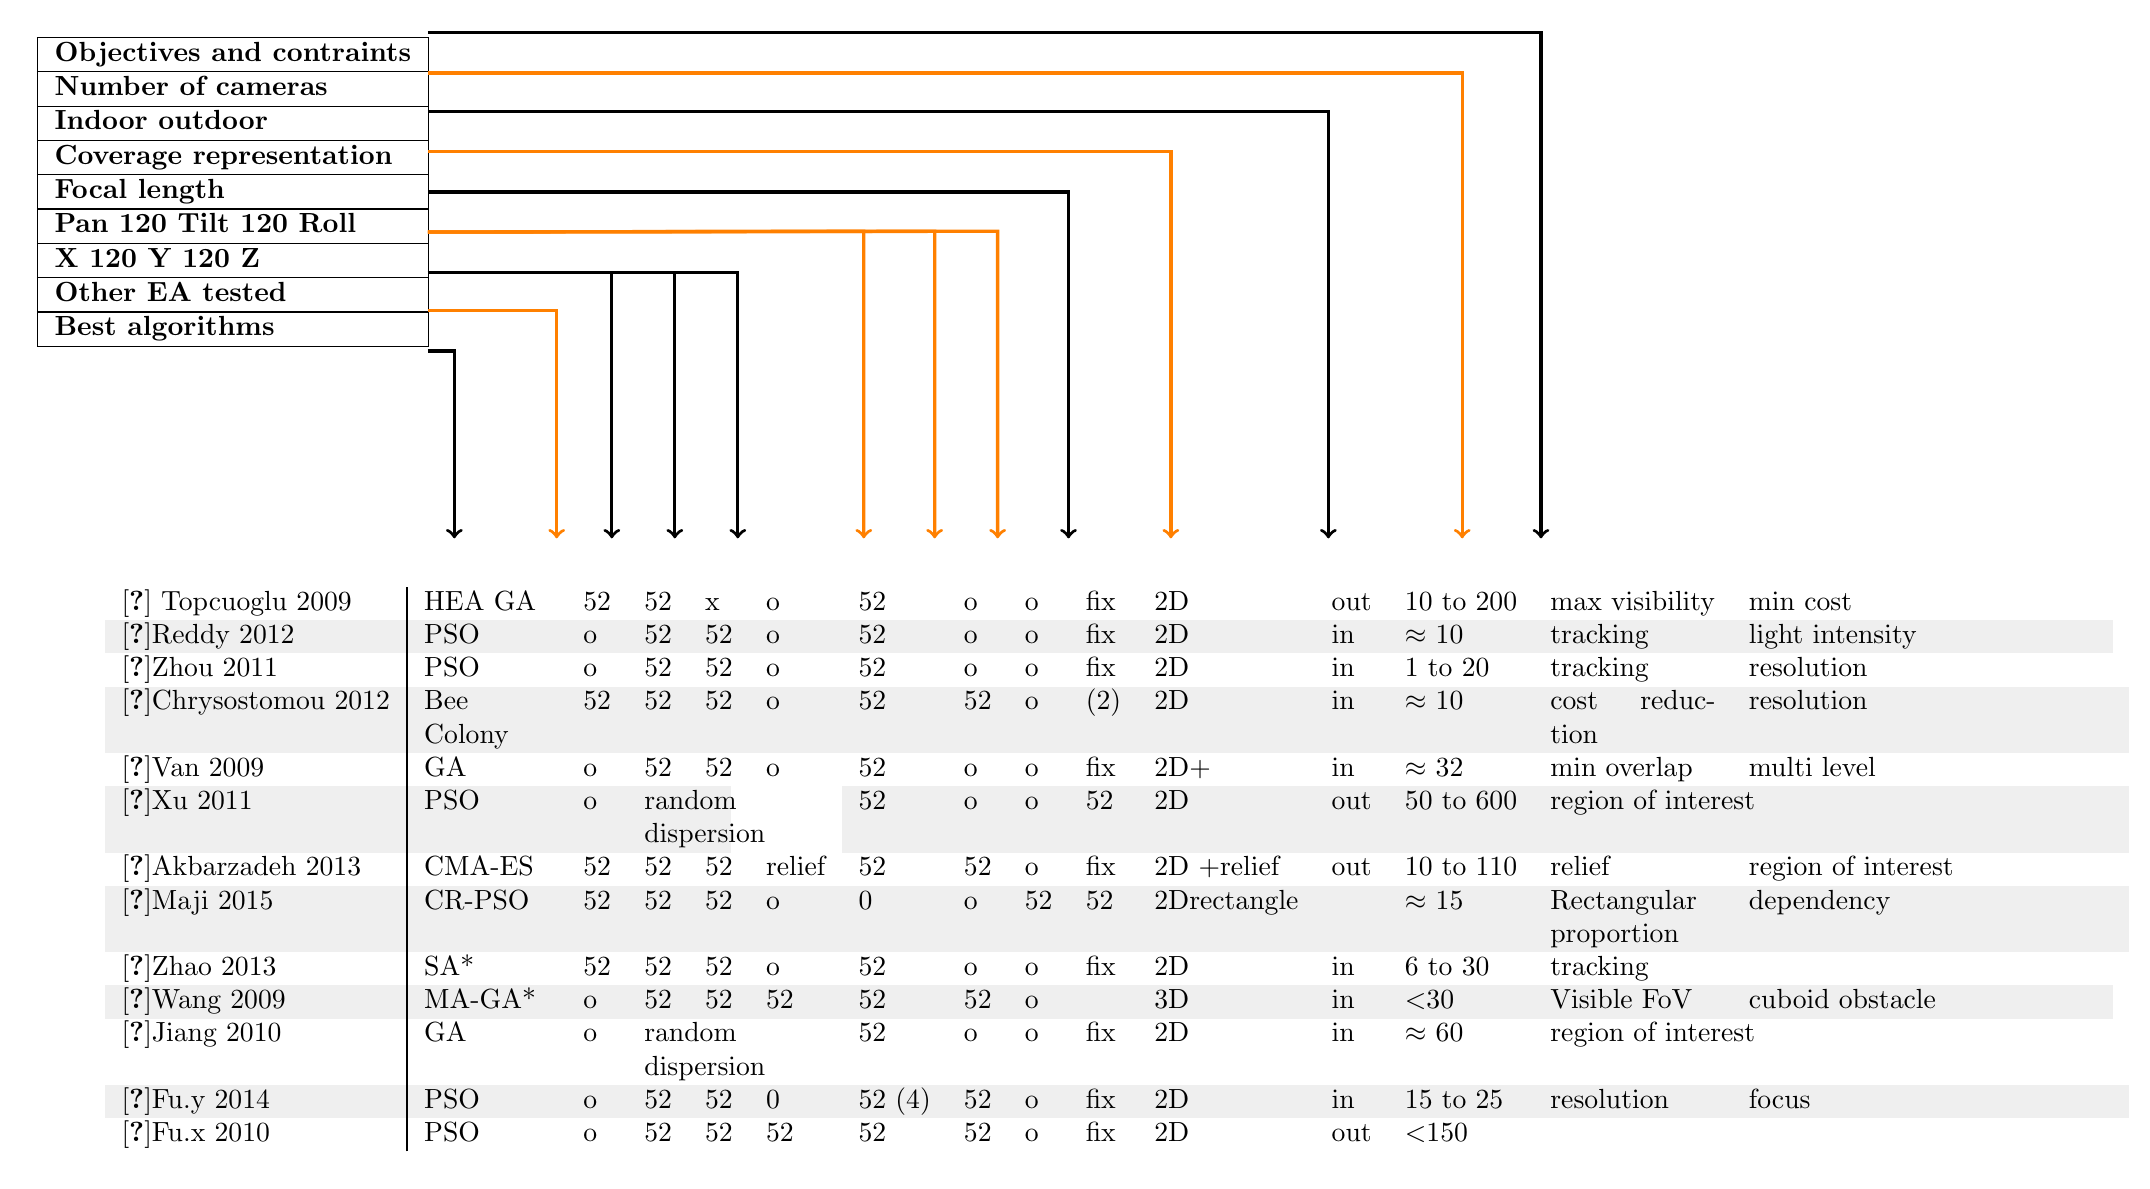
\begin{tikzpicture}[left]
\node (a) at (-0,-0)
{

\begin{tabular}{|l|}
\hline
 % \textbf{Reference} \\ \hline
%   \textbf{Best algorithms}   \\\hline %\vdots
%  \textbf{Other EA  tested}  \\\hline
%   \textbf{X \ding{120} Y \ding{120} Z}\\ \hline
%      \textbf{Pan \ding{120} Tilt \ding{120} Roll }\\ \hline
%         \textbf{Focal length }\\ \hline
%          \textbf{Coverage representation }\\ \hline
%          \textbf{Indoor outdoor }\\ \hline
%           \textbf{Number of cameras }\\ \hline
   \textbf{Objectives and contraints}  \\ \hline
    \textbf{Number of cameras }\\ \hline
    \textbf{Indoor outdoor }\\ \hline
    \textbf{Coverage representation }\\ \hline
    \textbf{Focal length }\\ \hline
    \textbf{Pan \ding{120} Tilt \ding{120} Roll }\\ \hline
    \textbf{X \ding{120} Y \ding{120} Z}\\ \hline 
    \textbf{Other EA  tested}  \\\hline   
    \textbf{Best algorithms}   \\\hline
\end{tabular}
};

\node[yshift=-6.51cm,xshift=24cm] (b) at (a.south) 
{
%%               ref  | soluce |EA soluc|x|y|z| pan | tilt |roll | focal |coverage|in out |nmb|
\begin{tabular}{@{} l|p{1.6cm}    l      l l l   l    l      l     l      l         l      l p{2.1cm}p{2.3cm} p{1.9cm}@{}}
\toprule
\rowcolor[HTML]{F2F2F2} 
%\textbf{ref V2}                                      & \multicolumn{1}{l|}{\cellcolor[HTML]{F2F2F2}\textbf{\begin{tabular}[c]{@{}p{1.59cm}@{}}Best \\ solution\end{tabular}}} & \multicolumn{1}{l|}{\cellcolor[HTML]{F2F2F2}\begin{tabular}[c]{@{}p{0.9cm}@{}}Other\\ EA  \\ solution\end{tabular}} & \multicolumn{1}{l|}{\cellcolor[HTML]{F2F2F2}X} & \multicolumn{1}{l|}{\cellcolor[HTML]{F2F2F2}Y}& \multicolumn{1}{p{0.659cm}|}{\cellcolor[HTML]{F2F2F2}Z}&\multicolumn{1}{l|}{\cellcolor[HTML]{F2F2F2}Pan}& \multicolumn{1}{l|}{\cellcolor[HTML]{F2F2F2}Tilt}& \multicolumn{1}{l|}{\cellcolor[HTML]{F2F2F2}Roll}& \multicolumn{1}{p{1.119cm}|}{\cellcolor[HTML]{F2F2F2}Focal length} & \multicolumn{1}{l|}{\cellcolor[HTML]{F2F2F2}\begin{tabular}[c]{@{}p{1.55cm}@{}}Coverage\\  represen-tation\end{tabular}} & \multicolumn{1}{p{1.56cm}|}{\cellcolor[HTML]{F2F2F2}Indoor outdoor} & \multicolumn{1}{l|}{\cellcolor[HTML]{F2F2F2}\begin{tabular}[c]{@{}p{0.9cm}@{}}Number\\ of \\ cameras\end{tabular}} & \multicolumn{3}{l|}{\cellcolor[HTML]{F2F2F2}\begin{tabular}[c]{@{}l@{}}Secondary \\objectives \\ and contraints\end{tabular}}                                                                \\ \midrule
\rowcolor[HTML]{FFFFFF} 
\multicolumn{1}{l|}{\cellcolor[HTML]{FFFFFF}\cite{101*topcuoglu2009} Topcuoglu  2009} & HEA GA                                                                                                         &  \ding{52}                                                                     &  \ding{52} & x                                              & o                                              &  \ding{52}                                                & o                                                 & o                                                 & fix                                                       & 2D                                                                                                              & out                                                          & 10 to 200                                                                                                 & max visibility & min cost         &                    \\
\rowcolor[HTML]{EFEFEF} 
\multicolumn{1}{l|}{\cellcolor[HTML]{EFEFEF}\cite{33*reddy2012}Reddy 2012}  & PSO                                                                                                            & o                                                                     &  \ding{52} &  \ding{52}                                              & o                                              &  \ding{52}                                                & o                                                 & o                                                 & fix                                                       & 2D                                                                                                              & in                                                           & $\approx$ 10                                                                                              & tracking                                                                                                                    & \multicolumn{2}{l}{\cellcolor[HTML]{EFEFEF}light intensity}      \\
\rowcolor[HTML]{FFFFFF} 
\multicolumn{1}{l|}{\cellcolor[HTML]{FFFFFF}\cite{8*zhou2011}Zhou 2011}   & PSO                                                                                                            & o                                                                     &  \ding{52}                                              &  \ding{52}                                              & o                                              &  \ding{52} & o                                                 & o                                                 & fix                                                       & 2D                                                                                                              & in                                                           & 1 to 20                                                                                                   & tracking                                                                                                                    & resolution                    &                                  \\
\rowcolor[HTML]{EFEFEF} 
\multicolumn{1}{l|}{\cellcolor[HTML]{EFEFEF}\cite{82*chrysostomou2012}Chrysostomou 2012}  & Bee \newline Colony                                                                                                     &  \ding{52}                                                                     &  \ding{52}                                              &  \ding{52}                                              & o                                              &  \ding{52}                                                &  \ding{52}                                                 & o                                                 & (2)                                                  & 2D                                                                                                              & in                                                           & $\approx$ 10                                                                                              & cost reduction                                                                                                              & resolution                    &                                  \\
\rowcolor[HTML]{FFFFFF} 
\multicolumn{1}{l|}{\cellcolor[HTML]{FFFFFF}\cite{83*van2009}Van 2009}  & GA                                                                                                             & o                                                                     &  \ding{52}                                              &  \ding{52}                                              & o                                              &  \ding{52} & o                                                 & o                                                 & fix                                                       & 2D+                                                                                                             & in                                                           & $\approx$ 32                                                                                              & min overlap                                                                                                                 & multi level                   &                                 \\
\rowcolor[HTML]{EFEFEF} 
\multicolumn{1}{l|}{\cellcolor[HTML]{EFEFEF}\cite{84*xu2011}Xu 2011}  & PSO                                                                                                            & o                                                                     & \multicolumn{3}{p{0.89cm}}{\cellcolor[HTML]{EFEFEF}random \newline dispersion}                                                                                    &  \ding{52}                                                & o                                                 & o                                                 &  \ding{52}                                                         & 2D                                                                                                              & out                                                          & 50 to 600                                                                                                 & \multicolumn{2}{l}{\cellcolor[HTML]{EFEFEF}region of interest}                                                                                              &                                 \\
\rowcolor[HTML]{FFFFFF} 
\multicolumn{1}{l|}{\cellcolor[HTML]{FFFFFF}\cite{141*akbarzadeh2013}Akbarzadeh 2013} & CMA-ES                                                                                                         &  \ding{52}                                                                     &  \ding{52}                                              &  \ding{52}                                              & relief                                         &  \ding{52} &  \ding{52}                                                 & o                                                 & fix                                                       & 2D + \newline relief                                                                                                     & out                                                          & 10 to 110                                                                                                 & relief                                                                                                              & \multicolumn{2}{l}{\cellcolor[HTML]{FFFFFF}region of interest}   \\
\rowcolor[HTML]{EFEFEF} 
\multicolumn{1}{l|}{\cellcolor[HTML]{EFEFEF}\cite{143*maji2015}Maji 2015} & CR-PSO                                                                                                         &  \ding{52}                                                                     &  \ding{52}                                              &  \ding{52}                                              & o                                              & 0                                                & o                                                 &  \ding{52}                                                 &  \ding{52}                                                         & 2D \newline rectangle                                                                                                    &                                                              & $\approx$ 15                                                                                              & Rectangular proportion                                                                                                            & dependency                    &         \\
\rowcolor[HTML]{FFFFFF} 
\multicolumn{1}{l|}{\cellcolor[HTML]{FFFFFF}\cite{151*zhao2013}Zhao 2013} & SA*                                                                                                            &  \ding{52}                                                                     &  \ding{52}                                              &  \ding{52}                                              & o                                              &  \ding{52}                                                & o                                                 & o                                                 & fix                                                       & 2D                                                                                                              & in                                                           & 6 to 30                                                                                                   & tracking                                                                                                                    &                               &                                  \\
\rowcolor[HTML]{EFEFEF} 
\multicolumn{1}{l|}{\cellcolor[HTML]{EFEFEF}\cite{152*wang2009}Wang 2009} & MA-GA*                                                                                                         & o                                                                     &  \ding{52}                                              &  \ding{52}                                              &  \ding{52}                                              &  \ding{52}                                                &  \ding{52}                                                 & o                                                 &                                                           & 3D                                                                                                              & in                                                           & \textless30                                                                                               & Visible FoV                                                                                                                 & \multicolumn{2}{l}{\cellcolor[HTML]{EFEFEF}cuboid obstacle}      \\
\rowcolor[HTML]{FFFFFF} 
\multicolumn{1}{l|}{\cellcolor[HTML]{FFFFFF}\cite{165*jiang2010}Jiang 2010} & GA                                                                                                             & o                                                                     & \multicolumn{3}{p{0.659cm}}{\cellcolor[HTML]{FFFFFF}random  \newline dispersion}                                                                                    &  \ding{52}                                                & o                                                 & o                                                 & fix                                                       & 2D                                                                                                              & in                                                           & $\approx$ 60                                                                                              & \multicolumn{2}{l}{\cellcolor[HTML]{FFFFFF}region of interest}                                                                                              &                                  \\
\rowcolor[HTML]{EFEFEF} 
\multicolumn{1}{l|}{\cellcolor[HTML]{EFEFEF}\cite{193*fu2014}Fu.y 2014} & PSO                                                                                                            & o                                                                     &  \ding{52} &  \ding{52} & 0                                              &  \ding{52} (4)                                            &  \ding{52}                                                 & o                                                 & fix                                                       & 2D                                                                                                              & in                                                           & 15 to 25                                                                                                  & resolution                                                                                                                  & focus                         &                                 \\
\rowcolor[HTML]{FFFFFF} 
\multicolumn{1}{l|}{\cellcolor[HTML]{FFFFFF}\cite{194*fu2010}Fu.x 2010} & PSO                                                                                                            & o                                                                     &  \ding{52}                                              &  \ding{52}                                              &  \ding{52}                                              &  \ding{52}                                                &  \ding{52}                                                 & o                                                 & fix                                                       & 2D                                                                                                              & out                                                          & \textless150                                                                                              &                                                                                                                             &                               &                                 
\end{tabular} };
\draw [->,very thick] 		  (-0.135,2.02) -- (14,2.02) -- (14,-4.4); % constraint
\draw [->,very thick][orange] (-0.135,1.51) -- (13,1.51) -- (13,-4.4); % nmb cam
\draw [->,very thick] 		  (-0.135,1.02) -- (11.3,1.02) -- (11.3,-4.4); %in out
\draw [->,very thick][orange] (-0.135,0.51) -- (9.3,0.51) -- (9.3,-4.4);% coverage representation
\draw [->,very thick] 		  (-.135,0.0) -- (8,0) -- (8,-4.4); % focal lengh
\draw [->,very thick][orange] (-.135,-0.51) -- (7.1,-0.5) -- (7.1,-4.4); % roll
\draw [->,very thick][orange] (-.135,-0.51) -- (6.3,-0.5) -- (6.3,-4.4); % tilt
\draw [->,very thick][orange] (-.135,-0.51) -- (5.4,-0.5) -- (5.4,-4.4); % pan
\draw [->,very thick] 		  (-.135,-1.02) -- (3.8,-1.02) -- (3.8,-4.4);  %z
\draw [->,very thick] 		  (-.135,-1.02) -- (3.0,-1.02) -- (3.0,-4.4); % y
\draw [->,very thick]		  (-.135,-1.02) -- (2.2,-1.02) -- (2.2,-4.4); % x
\draw [->,very thick][orange] (-.135,-1.51) -- (1.5,-1.51) -- (1.5,-4.4); %EA tested
\draw [->,very thick] 		  (-.135,-2.02) -- (0.2,-2.02) -- (0.2,-4.4); % best Al
\end{tikzpicture}
\end{table}
\end{landscape}



%%%%%%%%%%%%%%%%% exemple double  table arrow%%%%%%%%%%%%%%%%%%%%%%%%%%%%%%%%%%%%%

 
%%%%%%%%%%%%%%%%%%%%%%%%%%%%%%%%%%%%%%%%%%%%%%%%%%%%
%\subsection{Field of view}
%
% optical and the occlusion
%
%cover an area with certain amount of sensors. This number of position can be estimate as follow.\\   
%Each camera defined m focusing of optimize the solution and return a acceptable solution.
% 


%####################TODO############################
\section{Coverage path planning part  CPPP }

The solutions put forward in the literature until now to keep on eyes a vast area composed by numerous obstacles was to pose numerous cameras or robotics cameras (as PTZ cameras and smart camera).
The solutions proposed until now are interesting only to monitor a vast area  in continue with several cameras. 
The disadvantage of positioning a set of cameras appears quickly with the cost. The cost is due to the several cameras and the communication network required to can centralize the image collected. All the images must be collected in a real time. This costly system is not always useful. 
In fact, in some application the area needs to be controlled periodically. The periodic control of the area does not require an installation of the set of fixed cameras unlike the solution presented until now (see section \ref{sec:SolutionBasedonEA} and section \ref{sec:NonEAmethod}). The periodical control requirement can be illustrate with some example :  the cartographies with need just one fly over an area roughly bounded as in \citep{66*galceran2013} [164*], forest fire detection which require a periodic fly over specific and vast region as in [237*], the hoovering robots with need to cover all the room with some time some on-line computation [216* 218* 215* 196*] and the agriculture.
 About the agriculture application, an UAV need to fly over the field few time the year in order to control by photography the hydration, the maturity, etc, as in [203*,63*,105*,164*,167*,177*,203*]. %\textbf{revoir les ref et trié un peu}.

For all these applications the area must be covered but does not need a coverage of all the area instantly and continuously. The solution commonly proposed is to use only one sensor mounted on a mobile robot. Mobile robots need to be adapted to the task and the environment, as flying [105*], driving [213*,30*], swimming [66*]. The mobile robot with the sensor moves in the space to cover all the area. In this case, the objective is to determine the best path for the mobile robot to cover all the area. The best path is dependent then the constraint of each problem. However, the common point, is to have the shorter path to all or at least most of the area.
The following section is focused on finding the best Coverage Path Planing (CPP) for a sensor mounted on a mobile robot. The sensor can be varied, but the great majority of the case it is a camera perspective. To estimate the best CPP different algorithms and methodologies has been applied in the literature to solve or at least optimize the CPP problems.

  The following sections is focussed on the different algorithms and methodologies applied to solve or at least optimize the coverage path planning problem. In a first time, the watchman route problem is introduced to highlight the origin of the CPP problem and the relation with the cameras positioning for optimal coverage. In a second time, the more popular solutions are discussed.
 



%hovering robot
% In some case some domestic robots as  the hovering robot   or similar  must also to 213*


%-------------------------------------\\
% Grenzdorffer, G., Engel, A., Teichert, B.: The photogram-metric potential of low-cost UAVs in forestry and agriculture. Int. Arch. Photogram. Rem. Sens. Spatial Inform. Sci.
%31(B3), 1207–1214 (2008) 
%
%Zarco-Tejada, P.J., Berni, J.A., Suarez, L., Fereres, E.: A new era in remote sensing of crops with unmanned robots.
%SPIE Newsroom, pp. 2–4 (2008)
%
%Kazmi, W., Bisgaard, M., Garcia-Ruiz, F., Hansen, K.D.,
%la Cour-Harbo, A.: Adaptive surveying and early treatment
%of crops with a team of autonomous vehicles. In: European
%Conference on Mobile Robots, pp. 253–258 (2011) 





\subsection{AGP  to watchman route problem}


Before to explore the solutions proposed for the CPP is essential to understand the role of the Watchman route Problem (WRP). The WRP is closely related than the CPP and the WRP has impacted the research for the CPP. 
The following sections are focused on the definition of the WRP, the solution proposed in order to solve it, and finally a fast discussion of the limit of the WRP  is proposed.
 
\subsubsection{Definition of the watchmen problem }

The Watchman Route Problem is introduced for the first time by Chin and Ntafos in 1987 54* \cite{54chin} . The problem of the WMP can be summarized in one sentence :

\textbf{"How to calculate a shortest route contained inside a polygon such that any points inside this polygon is visible from at least one point of the route?"}.  

The guard has to cover an area represented by a polygon. The guards is considered as perfect with no restriction in the field of view (the guard can see at $360^\circ$) and no restriction in the depth field (the guard can see form on extremity of the room the guard can see the opposed wall until no obstacle look him). The guard ability are directly inspired by the AGP (see \ref{sec:AGP})
The shape of the polygon is primordial and affect greatly the possible answer and the complexity to solve the WRP.
The WRP problem is by many aspects closely related than the AGP. The AGP (see  section \ref{sec:AGP}) is commonly considered as the roots of the WRP.
 In fact, the WRP is not only focussed on fixing position but on finding an optimal path. The path has to be optimized to cover all the points which compose the polygon  and the path have to be shorter as possible.
 
% A common way to build a path with as to cover a polygon can be to search the waypoints  which compose the path. Once the waypoints found the next step is to compute a path passing by all the previously founded waypoints. 
 The next section introduces the possible method and algorithm usable in order to solve or atleast optimize a solution for a WRP.
 


%polygone impact on the complexity
%AGP -> WRP  

% source : An Approximate Algorithm for Solving the Watchman Route Problem Fajie Li and Reinhard Klette
 
\subsubsection{Solution} 

The WRP problem can be solve in some condition. The solution to solve it are applicable only if the polygon is simple. A polygon is considered as simple, when the boundary of it are composed of continue straight lines that do not intersect between them. To complete this definition, it is important to precise the simple polygon does not have a hole (see Figure \figref{fig:simplePoly}). 
 \begin{mfigures}[!]
{Few example to illustrate the simple polygon. }{fig:simplePoly} \centering
\mfigure{width=.4\linewidth}{img/SimplPolygonA.png}{Example of simple polygons.}{subfig:SimplePoly}
\hspace{1cm}
\mfigure{width=.4\linewidth}{img/SimplPolygonB.png}{Example of non simple polygons.}{subfig:nonSimplePoly}
\hspace{1cm}
\end{mfigures}	

To solve the WRP few algorithms were developed. Step by step the algorithms proposed in the literature allow a faster solution. The first interesting algorithm for the WRP with the simple polygon is the early work of Tan, X [234*]\cite{}. In [234*] propose an algorithm for a fast computation time. The solution proposed work in the simple polygon composed by $n$ vertices in a polynomial time $O(n^5)$. \\
Others algorithms proposed to go a bit further. Dror et al [233*]\cite{} assume to have a better  time complexity. In fact, in [233*]\cite{} the solution proposed for the WRP in a simple polygon is working in $O(n^3 log n)$.  The deterministic solution applied is also usable in closely relate problem of the WRT as the zoo-keeper problem and safari problem.
This two algorithms [233*][234*] are usable only in the case of simple polygon to delivered the optimal solution which is the shortest path for the full room coverage. 

To have a more general solution for WRP, the proposition is to have an efficient algorithm working also in the complex polygon. A solution is to look for an efficient approximation. An efficient approximation means a path short enough.  Due to the computation method the optimality of the path can not be certified as the best.
Several efficient approximations has been proposed as in [235*] and [53*]. 

In Packer [53*] the algorithm proposed is based on splitting the problem into two sub-problems. The first sub-problem is to find a set of points with can be good enough to cover all the area despite a restricted visibility range. These points are called waypoints.  
Once the set of waypoints to cover all the polygon are found, the second sub-problem is to create a path passing by all this points. 
 This second sub-problem is similar then a classic Travelling Salesman Problem (TSP). The TSP try to answer the questions asks by a travelling salesman "\textbf{What is the shortest path passing by each city only one time and return to the starting city?}".
  In the TSP, the cities are the node on the interconnected map and the roads are the connexion between them. The TSP is a well known as NP-hard and NP-complete in the some condition as described in [236*]. \\ 
Finally the solution used for the TSP can be applied for the second sub-problem of WRT.
 The TSP and the algorithms proposed to optimize it are discussed more in detail later \ref{par:TSPPathPlan}

%a similar method than the one proposed by faigl in [235*] has been proposed to approximate the shorter path as possible. To approximate the shorter path the problem of WRP is also split in two sub-problem. The first sub-problem is considered as similar then the AGP and use the method form AGP to find the waypoints. The second sub-problem is also compared as TSP.

In faigl [235*] a similar method than the one proposed by Packer [53*] has been proposed to approximate the shorter path as possible. The problem is also split into two sub-problems with the first is to optimize the position of the waypoints and the second is to schedule the position in order to create a path planning (directly inspired by the TSP). 
%the algorithm proposed is based on splitting the problem into two sub-problems. The first sub-problem is to find a set of point with can be good enough to cover all the area despite a restricted visibility range. These points are called waypoints for the following sections. 
 Furthermore, the solution proposed by Faigl in [235*] is applicable to a watchman with a restricted visibility range. Equivalent then a $360^\circ$ field of view with a restricted depth of field. This restriction affects greatly the waypoints positioning.
 Once the set of waypoints to cover all the polygon is found, the second sub-problem is to create a path passing by all this points.  The algorithms proposed  to do it, are also inspired by the solution given for the optimize the TSP.
 %This second sub-problem is similar then a classic Travelling Salesman Problem (TSP). The TSP  try to answer the question ask by a travelling salesman "What is the shortest path passing by each city only one time and return to the starting city?". In the TSP, the city are the node on the interconnected map with the road as the connexion. The TSP is well known as NP-hard and NP-complete in some condition as described in [236*]. \\ 
%Finally the solution used for the TSP can be applied for the second sub-problem of WRT.
% The TSP and the algorithms proposed to optimize it are discussed more in detail later \ref{par:TSPPathPlan} \\
%In Packer [53*] similar solution than the one proposed by faigl in [235*] has been proposed to approximate the shorter path as possible. To approximate the shorter path the problem of WRP is also split in two sub-problem. The first sub-problem is considered as similar then the AGP and use the method form AGP to find the waypoints position. When the  waypoints are placed in the polygon the second sub-problem which is to schedule the waypoints to have a shorter path as possible. 



%from https://link.springer.com/content/pdf/10.1007%2F978-3-642-31155-0.pdf
%compexity $O(n^4 log n)$ :\\
%Dror, M., Efrat, A., Lubiw, A., Mitchell, J.S.B.: Touring a sequence of polygons.
%In: Proc. 35th Symposium on Theory of Computing, pp. 473–482 (2003)\\
%Tan, X.: Fast computation of shortest watchman routes in simple polygons. Information Processing Letters 77(1), 27–33 (2001) \\ 

%linear approximation :  Tan, X.: A linear-time 2-approximation algorithm for the watchman route problem for simple polygons. Theoretical Computer Science 384(1), 92–103 (2007)

%Polygons with holes the problem is NP-hard : 54*\\
 %  Dumitrescu, A., T oth, C.D.:Watchman tours for polygons with holes. Computational Geometry: Theory and Applications  (2012)

 %An $O (log n)-approximation$ for Rectilinear polygons are also known as orthogonal polygons.:Mata, C.S., Mitchell, J.S.B.: Approximation algorithms for geometric tour and network design problems. In: Proc. 11th Symposium on Computational Geometry, pp. 360–369 (1995)

\subsubsection{Limit and consequences}

The method proposed to solve the WRP are really interesting and give a good solution in some specific condition. This condition are the limit of the method proposed. In fact the optimal solution, that mean the shortest path which cover all the area (polygon) are usable only if the polygon respect some rule. The polygon must be simple.  \\
When the polygon begin to be more complex the optimal solution cannot be reached. The method applied to solve the WRP for complex area are interesting. Especially in the splitting the problem into sub-problem. Despite this interesting aspect the solution proposed are most of the time limited due to the area representation (must be a polygon composed by vertex). This representation associate to the geometric methodologies to find the waypoints give an crucial importance to the number of vertex in relation then the number of cameras. More the number of vertex is important more the first sub-problem will be difficult and long to solve. 
Consequently this method is not the more appropriate for the vast and complex outside area which would require  numerous vertex to describe it.
 The biggest limit of the WRP is the ability of the watchman. In fact in the original problem, the Watchman is considered has perfect visibility. The solution proposed for answer to the WRP are not usable when some constraint is added in the  visibility. 
In Faigl [235*] the WRP begin to be extended by add a constraint on the visibility. In this condition the problem is slightly muted to self-organizing map  in the way to became a coverage path planning.

The AGP then WRP has greatly impacted the vision and the problem design of cameras coverage and coverage path planning. Especially the CPP by splitting the problem into two sub-problem.  



 


%tout comme l'agp a était une source d'inspiration pour  le positionnement de camera  le wmp est lui aussi une source d'inspiration pour  le cpp 
%The CPP 
%The origin of CPP can be found on the Watch Men Problem (WMP). The next
%
%The Watch Men Problem (WMP) is directly derived form the AGP. 
%
%As the importance of AGP for the problem of camera positioning  the Watch men problem 
%53* parcker eli :  propose a solution  to solve the watchmen problem based on the result optianined by the AGP \\ 
%54* Chin : complexity proof of NP-hard  for the watchmen problem by reduction of TSP + article fondateur
%

\subsection{CPP solutions}

To optimize the CPP problems many solution was been proposed. The different algorithms and methodologies proposed are discussed in the following sub-section. The methodologies proposed can be split in several branches. 
The more important methodologies to optimize the CPP is  the use of sweep associate to a cellular decomposition.
%60* =  une découpe en zone  rectangle et utilisation  de la triangulation pour le positionment de waypoint  puit tsp.
%
%217*= utilisation du GA  pour la conexion entre polygone simple (1er étape découpe de la zone  en  polygone en fonction des obstacle - 2e  crée un graphe qui  reli les différant sous partie ( polygone) GA  -3 choisir le sweep le plus )
%
%61* 62*= floor planning

\subsubsection{ Cellular decomposition and sweep}
To solve the CPP problem the solution the most common is to use the cellular decomposition. The cellular decomposition is  by some aspect inspired by the methodologies presented from the WRP.
To remember one of the interesting solution for the WRP  is to split the problem in two sub-problem and optimize its independently. The first sub-problem is to find the best waypoints and the second sub-problem is to find the shorter path passing by all the waypoints (as a TSP).
 The Cellular decomposition also split the problem of CPP in two sub-problems. The first sub-problem is focus on the decomposition of the complex area in several cells.  Each cell has to be a simple polygon (basically a rectangle or latter any quadrilateral polygon). Inside each cell a sweep will be applied in order to cover all the area. The second sub-problem is to find the path which can connect each simple polygon. The problem has to take in account in many case the sweep start and end to find the global shorter path. where the global shorter path  take in account the sweep trajectory of each simple polygon and the path between the  simple polygons.
 
 Finally the cellular decomposition is made by the decomposition of the complex area, choose the appropriate  sweep and find the shorter path to connect the cells. 
 
 \paragraph*{Decomposition}\label{par:decomposition}

 The decomposition in cells has to objective to split the a complex area in several sub-area. The sub-area has to be simpler in term of shape in order to can applies a sweep. 
Since the 90s numerous algorithm has been developed for the cellular decomposition. Among the algorithms for cellular decomposition, 3 type of decomposition has been made in the survey of choset [214*]and \cite{66*galceran2013}. 
\begin{itemize}
	\item Approximate: 
		An approximate decomposition is based on a discretization of the area. The free space of the area is representative by a set of case (gird). Each case of the grid has to be cover by the mobile robots.  The case is considered  completely cover if the robot is on this position. That mean the frequency of the grid is defined by the covered area of the mobile robots. 
		The approximate decomposition by case is fast to describe the area but is greatly limited due to the low sampling frequency of the gird and the limited trajectory possible.\\
	 
	\item Semi approximate: 
	 The semi approximate decomposition is by part based on the discretization of the space. The idea is to create a set of large cells. The width of the cells is fix and the height is relative then the area boundary. 
	 The semi approximate cell decomposition allow to have cells with two parallel side  with a fix size  (at the right and left) and  the  two other side adapted to the boundary (at the up and down).  The width  of  the cell chosen depending then half of the focal length of the camera mounded on the mobile robot. The area is covered by following the boundary of the cells with sweep to pass cells  after cells.
	 The advantage of this semi approximate decomposition is the facility to describe a vast area and the low computation required. Additionally this decomposition can be made on-line by the robot and do not require a hight level of knowledge of the area. The disadvantage is the non optimized path due to the cell decomposition. The simplicity  of this decomposition  can gender case where the robot have to path many time by the same place. The semi approximate cellular decomposition do not allow to have an optimised path planning. 
	 %%%%% add fig from238* fig8 to --> from214
	\item Exact cellular decomposition: 
	The exact cellular decomposition describe the area by create juxtaposed geometrical region. The size of the region (or cells) are not dependent then the robots ability despite the previous decomposition. The large size of the cell allow the  mobile robots to  do back and forth motion to cover all the cell (also called sweep).  The cells have to be ordered to have an efficient and short path passing by all the cells. The path has to limit the distance to pass  between the cells.
	The exact cellular decomposition became popular and numerous algorithms has been proposed to has  a faster decomposition and with a more appropriate shape depending then the area shape. 
	Among the numerous exact cellular decomposition the trapezoidal decomposition for this simplicity and historic importance, the Boustrophedon decomposition  and  Morse-based Cellular Decomposition for their important in the construction of other exact cellular decomposition has to be cited. These algorithms and other has been clearly summarized in the survey of Carreras and Galceran \citep{66*galceran2013}. 
	The exact cellular decomposition has continue to be studied since the survey of  Carreras and Galceran  \citep{66*galceran2013} and upgraded, as in 144* for propose a decomposition for concave or multiple polygons.
	
\end{itemize}




% survey = 66* 214*
% CPP experimentation (164* 167*)
% 
%119* 214* 215* 146*  144* 164* 167* 190*=cellule decomposition \\ 

 
 \paragraph*{Sweep} \label{par:sweep}
	The back and forth or sweep is an essential element of the CPP by cellular decomposition. The sweep has to cover the entire cell.s The cells are splitting the area in relatively simple polygon (as see in the paragraph \ref{par:decomposition}). The sweep has to be adapted then the shape of the cells and also must start and finish in a appropriate position for passing to the next cell.
	For that the starting point of the sweep and the ending point are crucial for the global path planning.
	In Torres et al 144* the sweep is function then a direction and can go clockwise or counter-clockwise to have a start and end in the appropriate position for the transition. 
	 This allow to have 8 different  applicable sweeps at each cell depending then the more appropriate start and finish. The sweep  are adapted depending then : the turn side ( clockwise or counter-clockwise), the direction (horizontal or vertical) and the finishing  position (start and stop form the same side or opposite side).  
	 The sweep can be also alternatively switch for a spiral as proposed in Jimenez et al [217*]. The proposed sweep and spiral in [217*] are adaptable depending then the context. The sweep can have two direction and for the spiral two turn side (clockwise or counter-clockwise).
	 
	To have an adapted sweep the footprint has to be defined depending then the camera ability and the objective. In 144* the size of the sweep is dependent then the area cover by a camera and a sufficient amount of overlap for the 3D reconstruction (see also [191*]). In Li et al  \citep{146*li2011} the foot print of the camera with a small pan is take in account. Due to the pan the camera projection is not a rectangle but a trapezoid. Consequently the sweep size is adapted by taking the larger side of the trapezoid for the sweep dimension.
	Also for the grid decomposition the sweep size is directly related the coverage ability of the mobile robots (as example in [215*][195*]).  % also 216*+48  215*  195* +55 218*+12  use a sensing camera at the front).
	
	One extra element to take in account for the sweep can be in some case the external element as the wind. In [215*][190*] the external condition are taking in account in the cost function and influence the sweep.
	
	
	To summarize the sweep as to be adapted then the area and the relation between cells. To choose the appropriate sweep the following element has to be taking in account:
	\begin{itemize}
		\item The size of  sweep  has to be defined depending then the ability of the camera (foot print size).
		\item The direction (horizontal or vertical).
		\item The finishing  position (start and stop form the same side or opposite side)
	\end{itemize}
To  can has the more appropriate sweep is primordial to know by advance  the cells scheduling when is needed. The cells scheduling is the main part of the path planning.

	% The foot print, 
	 %the type of sweep ( sweep or spiral), the direction (horizontal or vertical), the finishing  position (start and stop form the same side or opposite side) the size of the footprint has to be defined depending then the ability of the camera. 
	
	%215* 190* generic cost depending then external condition  and  using spiral or sweep
	 
	 %144*  size to the sweep adapted  depending then the footprint of the camera on the ground floor  with propose lot of overlap useful for the 3D reconstruction.  the sweep  is function then a direction  and can go  clockwise or counter-clockwise to have  a start and end in the appropriate position for the transition. 
	 %This allow to have 8 different sweep applicable at each cell depending then the more apropriate start and finish depending  then the turn side ( clockwise or counter-clockwise), the direction (horizontal or vertical)  and the finishing ( start and stop form the same side or opposite side).  
	% 217*  propose  sweep and spiral with  different direction  for the sweep and two turn side for the  spiral

	%195* spiral sweeping for on-line coverage (for hoover application)
	 
%	209* comparative between cellular decomposition with sweep and a global spiral on the complex shape. (master these)
	
	
    
 
 %décompostion celulurai avec étude sur le remplisage sweep ou  spyrale pour  des zone concave our convex 
%Ost, G.: Search Path Generation with UAV Applications Using Approximate Convex Decomposition, Masters Thesis. Linkopings universitet, Sweden (2012)

 
 \paragraph*{Path planning} \label{par:TSPPathPlan}
 
 The path planning as to aims to find the short path passing by all the cells. The path planning became even more tricky in the case of exact cellular decomposition. Or for any decomposition which requires a sweeping inside each cells. In fact in this case, the goal is to have the shorter path planning with taking in account each sweep and transition between cells. In the precedent paragraph \ref{par:sweep} the sweep has been detailed.
 To find the best scheduling between each cells the algorithm form the TSP are commonly used.     
 
 When the area are decomposed in cells the goal is to schedule the priority of passage from one cell to another in order to create an efficient path passing by all the cells. The scheduling of the cells can be solved to use the paradigm of TSP (Traveling Salesman Problem) to have a path planning. 
The TSP is well known problem and is  deeply studied form long time ago.  First is essential remember the TSP is an NP-complete and NP-hard problem as proofed in KARP in [236*]. 

To optimize the TSP numerous algorithms was tested and some of them has been specially applied to schedule the cells to have the shorter path. In [60*] two methods was tested before to develop a third. The method used are based on branch and bound algorithms and develop a method called "Novel Previous-Next Waypoints Coverage Constraint" (PNWCC). The algorithms presented in [60*] propose at same time a schedule of each cells with also a smooth trajectory without sharp edges usable for non holonomic driving robots. 

	In the survey of Carreras et Galceran \citep{66*galceran2013} among the solutions proposed to solve the   TSP is to computes an exhaustive walk trough the adjacency graph. This solution is workable only for small adjancy graph. Among the other solution proposed the Genetic Algorithm. The GA is popular to optimize the TSP and is comonly use to evaluate the influence of this parameter as in \citep{68*muhlenbein1989} \citep{80*serpell2010} [139*]. About the CPP problem the GA is used to optimize the TSP in JIMENEZ et al [217] after a exacte cellular decomposition of a complex polygon. 
	
The GA is announced well appropriate to have an optimized solution for the TSP. 
Also the in some situation a  TSP is not realistic and some external constraint can be added as the wind effect, the turbulences, or holonomy constraint (see [102*,56*,66*] \citep{66*galceran2013}).
 
 
%236* proof of NP complet and NP-hard

%60* use of TSP = any TSP algorithm can be used  as the branch and bound algorithm. or best choice is to use  the Hearest Neighbor algorithm  and finally propose a Novel PNWCC solution with propose a path without  sharp edges usable for non holonomic driving robots.
%66* TSP  solver with a  several methode. 
%217* use of TSP  solved with GA (CPP)217*  GA  for the TSP

%102* TSP with external constraint (wind)
 
%68* asyncorne parallel GA for TSP
%80* GA mutation rate for TSP 
%139* GA config for TSP
%172* TSP GA   Use of GA multi goal for  schedule the charge on  m machine and n job  

%XX 56* evitement d'obstacle et trachectioire 
%XXX 214* reference of the problem 
%XXX 164*  use TSP 


\subsubsection{Other solution for CPP}

%
%In choset et al 214*  some heuristic and randomized solution has been presented.    
%one of the basic heuristic is to follow the boundary of the area to cover. (R.A. Brooks, A robust layered control system for a mobile robot, IEEE J. Robotics Autom. (1986)   et
%  E. Gat and G. Dorais, Robot navigation by conditional sequencing, in: Proc. IEEE Int. Conf. on
%Robotics and Automation, San Diego, CA (May 1994) pp. 1293–1299. )
%
%	\begin{itemize}
%	\item Liu, Y., Lin, X., Zhu, S.: Combined coverage path planning for autonomous cleaning robots in unstructured environments. In: Proc. World Congress on Intelligent Control and Autom., pp. 8271–8276 (2008) 
%
%	\item Luo, C., Yang, S.X.: A bioinspired neural network for
%real-time concurrent map building and complete coverage robot navigation in unknown environments. IEEE
%Trans. Neural Netw. 19(7), 1279–1298 (2008) == PDF TNN2008  cite 132  neural network pour  robot aspirateur  avec construction de la map  et complet couverture  
%	
%	\item Oh, J.S., Choi, Y.H., Park, J.B., Zheng, Y.F.: Complete coverage navigation of cleaning robots using
%triangular-cell-based map. IEEE Trans. Ind. Electron. 51(3), 718–726 (2004) == pdf navigation-robot.pdf   robot roulant construction de son univer ajout de direction possible
%
%	\item 214* = propose 2 heuristic  et randomize 
%	\end{itemize}
	
	216* 218* 215* 196*= robot roulant hoover \\
	
	191* 190* 211* 212* = low enregie cpp\\
%	177*= multi spectral\\
%	119* 214* 215* 146* 66* 144* 164* 167* 190*=cellule decomposition \\
%	146* 147* = optimization de trajectoire local cpp\\
%	196* =neural Network \\
%	195* 189*= ???
%
%%\subsubsection{ ??sensor positioned in electronic circuit ??}
%%\subsection{Robot application}
%	%\subsubsection{hover robot}
%	%\subsubsection{submarine}
%	
%	
%	!!!!!!!!!!!!!!!!!!!!!!resource!!!!!!!!!!!!!!!!!!!!!!!!!!!!\\ 
%	from 190
%
%\subparagraph{Probelm du CPP par Genetic Algo GA }	
%\begin{itemize}
%	\item Jimenez, P.A., Shirnzadeh, B., Nicholson, A., Alici, G.: Optimal area covering using genetic algorithms. In: Proc. IEEE/ASME Int. Conf. Advanced Intelligent Mechatronics, pp. 1–5 (2007)
%	
%	\item Wang, M., Tan, S., Yan, L.: Complete coverage path planning of wall-cleaning robot using visual sensor. In: Proc. Int. Conf. Electronic Measurement and
%Instruments, pp. 159–164 (2007)
%
%	\item Zhang, G., Ferrari, S., Qian, M.: An information
%roadmap method for robotic sensor path planning. J. Intell. Robot. Syst. 56(1–2), 69–98 (2009)
%	\end{itemize}
%
%
%\subparagraph{CPP  résolution par  neural Network pour certain une gestion dinamique de obstacle  }	
%\begin{itemize}
%	\item Lee, T.K., Baek, S.H., Oh, S.Y., Choi, Y.H.: Complete coverage algorithm based on linked smooth spiral paths for mobile robots. In: Proc. Int. Conf. Control, Automation, Robotics and Vision, pp. 609–614 (2010)
%
%	
%	\item Yang, S.X., Luo, C.: A neural network approach to complete coverage path planning. IEEE Trans. Syst. Man Cybern. 34(1), 718–725 (2004)
%
%
%
%	\item Luo, C., Yang, S.X., Stacey, D.A., Jofriet, J.C.: A solution to vicinity problem of obstacles in complete coverage path planning. In: Proc. IEEE Int. Conf. Robotics
%and Automation, pp. 612–617 (2002)
%
%\item Qiu, X., Song, J., Zhang, X., Liu, S.: A complete coverage path planning method for mobile robot in uncertain environments. In: Proc. World Congress on
%Intelligent Control and Automation, pp. 8892–8896 (2006)
%
%
%\item Qiu, X., Liu, S., Yang, S.X.: A rolling method for 
%complete coverage path planning in uncertain environments. In: Proc. IEEE Int. Conf. Robotics and
%Biomimetics, pp. 146–151 (2004)
%
%\item Luo, C., Yang, S.X., Stacey, D.A.: Real-time path planning with deadlock avoidance of multiple cleaning
%robots. In: Proc. IEEE Int. Conf. Robotics and Automation, pp. 4080–4085 (2003) 
%
%	\end{itemize}
%
%\subparagraph{survey  sur la décomposition  linaire }
%	\begin{itemize}
%	\item Choset, H.: Coverage for robotics-a survey of recent results. Ann. Math. Artif. Intell. 31, 113–126 (2001)
%	
%	\end{itemize}
%	
%	\paragraph{66*  points clé}
%	coverage path planning in the 3D space (UAV and Subamrine)\\ 
%	cellular decomposition :  requantangle cellul  ;  trapezoidal decomposition ; Boustrophedon Decomposition; Morse-based Cellular Decomposition ; online Morse-based Boustrophedon Decomposition ; Landmark-based Topological; slice Decomposition ;On-line Topological Coverage Algorithm ;Contact Sensor-based Coverage of Rectilinear Environments;Grid-based Methods;Grid-based Coverage using the Wavefront Algorithm;Neural Network-based Coverage on Grid Maps
%Coverage 
%		\paragraph{214* choset}
%		heurisitc and randomized approche :  propose a solution  on multi robot repultion system to spread the  robot  in the space and  use   a random motion  as strategie to explore the area[5,27]. \\(T. Balch and R.C. Arkin, Communication in reactive multiagent robotic systems, Autonom. Robots 1995) , unknown obstacles of arbitrary shape, Algorithmica 2 (1987) 403–430. ;:;\\ D. MacKenzie and T. Balch, Making a clean sweep: Behavior based vacuuming, in: AAAI Fall Symposium, Instationating Real-World Agents (1996). )
%		
%		\paragraph{Semi-approximate}
%		Hert and Lumelsky : propose a system based on cell decomposition  and   boundary folowing 
%		
%		\paragraph{multi robots}
		
		